\chapter{Fundamentals Of Distributed Data-Systems}
\label{chapter_technical_foundation}
\setlength{\epigraphwidth}{0.95\textwidth}
\setlength\epigraphrule{0pt}
\epigraph{\itshape ``I'm not telling you it's going to be easy - I'm telling you it's going to be worth it.''}{--- Arthur L. Williams Jr., \textit{Founder of Primerica Financial Services}}

In this chapter we will go trough the foundation of data-systems, requirements and concepts which apply to any (data-driven) system. This covers in particular following topics:
\begin{samepage}
\begin{itemize}
	\item Section \ref{tf_nfreq} Requirements of \textbf{\nameref{tf_nfreq}}, e.g. 
		\begin{itemize}
			\item \ref{tf_nfreq_scalability} \nameref{tf_nfreq_scalability}, 
			\item \ref{tf_nfreq_avrel} \nameref{tf_nfreq_avrel}, 
			\item \ref{tf_nfreq_maintainability} \nameref{tf_nfreq_maintainability}.
		\end{itemize}
	\item Section \ref{tf_storageconcepts} \textbf{\nameref{tf_storageconcepts}} for databases
	\item Section \ref{tf_dma} \textbf{\nameref{tf_dma}} concepts
	\item Section \ref{tf_dds} \textbf{\nameref{tf_dds}}, e.g.
		\begin{itemize}
			\item \ref{tf_dds_partitioning} \nameref{tf_dds_partitioning}, 
			\item \ref{tf_dds_replication} \nameref{tf_dds_replication}, 
			\item \ref{tf_dds_transactions} \nameref{tf_dds_transactions}, 
			\item \ref{tf_dds_consistency} \nameref{tf_dds_consistency} amongst others.\\
		\end{itemize}
\end{itemize}
\end{samepage}

At the end you will have a basic understanding about the difference between common and distributed systems and databases, the basic concepts of each of them and which one theoretically fits best to solve a certain problem.
A more hands-on deep-dive into related software, frameworks as well as specific problems and use cases will be demonstrated later in chapter \ref{chapter_software_frameworks} \nameref{chapter_software_frameworks}.

\section{Non-Functional Requirements Of Data-Systems}
\label{tf_nfreq}
When we think about data-driven systems, we mostly think about the same requirements we expect of any other data system we already know:
\begin{itemize}
	\item \textbf{Data Storage}: We need to store data and also need to be able to find it again later (\textit{database}). 
	\item \textbf{Data Querying}: We need to be able to query and filter data efficiently in certain kinds of ways (\textit{transaction and indices}).
	\item \textbf{Retention and Performance}: We want results fast, especially of expensive read operations (\textit{caching}).
	\item \textbf{Data Processsing}: We want to be able to process a huge amount of data (\textit{batch processing}) as well as process data asynchronously (\textit{stream processing}).\\
\end{itemize}

This sounds quite obvious, but remember those requirements are still the same as for the first database CODASYL\footnote{https://en.wikipedia.org/wiki/CODASYL} back in the 1960's. Even though there are and have been a lot of databases back in time, each of them with a diverse purpose and different approaches to solve e.g. indexing or caching - all of them still match those same requirements. Certainly those data systems evolved much further, especially within the last years, you may noticed:
\begin{itemize}
	\item Relational Databases being able to handle NoSQL data (e.g. even ``retirees'' like IBM DB2\footnote{\cite{IBMDB2JS}, https://www.ibm.com/support/knowledgecenter/en/SSEPEK\_11.0.0/json/src/tpc\\/db2z\_jsonfunctions.html} or Oracle\footnote{\cite{ORCLJS}, https://docs.oracle.com/database/121/ADXDB/json.htm}) as well as NoSQL databases being able to handle traditional SQL (e.g. ToroDB\footnote{\cite{TORODB}, https://www.torodb.com}) or
	\item databases becoming message queues (e.g. RethinkDB\footnote{\cite{RDBMQ}, https://rethinkdb.com/docs/changefeeds/} or Redis\footnote{\cite{RUDMQ}, https://redis.io/commands/rpoplpush}\footnote{\cite{BSARN}, see 5. Adopting Redis for Application Data}) and the other way around message queueing systems become databases (e.g. Apache Kafka\footnote{\cite{KFKQU}, https://kafka.apache.org/10/documentation/streams/developer-guide/interactive-queries.html}).\\
\end{itemize}

As you can see, boundaries between traditional databases and data-driven applications get blurred and in the same way more diversified. 
There is no one-size-fits-all solution, e.g. like you can find back in the past in the 1990's or early 2000s. 
At that time monolithic single-, 2 and 3-tier, architectures were state-of-the-art (see Figure \ref{schema_application_architectures} left-hand side). \\
Usually the \textbf{database layer} was represented by a data store like MySQL, Oracle, DB2 or even just files containing data stored on the local disk.\\
The \textbf{application layer} was usually a monolithic application developed in languages like PHP, Perl, C++ or Java and running on a web- or application server (e.g. Apache HTTP Server or IBM WebSphere).\\
And last but not least the \textbf{client layer}: a web browser like nowadays.\\
\begin{figure}[ht]
	\centering
  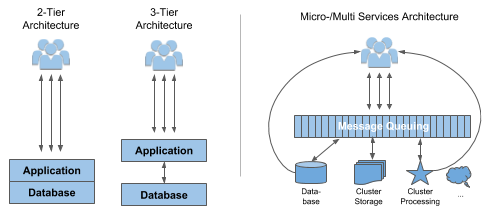
\includegraphics[width=1\textwidth]{application_architectures.png}
	\caption{Schema - Application Architectures}
	\label{schema_application_architectures}
\end{figure}
If you take a look at Figure \ref{schema_ebay_architecture_1997_1999} on page \pageref{schema_ebay_architecture_1997_1999} you can see an example of this time you may know: ebay.com. They have used the classical 3-tier architecture as well: Oracle as the database running on Solaris as OS\footnote{OS, Operating System}\abk{OS}{Operating System}, C++ as application code running on the Microsoft IIS\footnote{\cite{IIS}, \textit{Microsoft Internet Information Services, an extensible web server created by Microsoft for use with the Windows NT family.}} web server.
\begin{figure}[ht]
	\centering
  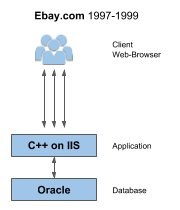
\includegraphics[width=0.4\textwidth]{ebay_architecture_199799.png}
	\caption{Schema - Architecture Ebay.com (1997-1999)}
	\label{schema_ebay_architecture_1997_1999}
\end{figure}
As you can already guess, this architecture won't scale very well today, in fact the only way to scale this application was to upgrade the single server (\textit{scale up vertically}), in case of ebay.com they once switched from commodity hardware to a very pricey mainframe server (Sun Enterprise E10000\footnote{\cite{EBAYA}, slide 11}) to buy some time. But as you may have noticed there are much more ovious issues, e.g. if you think about:
\begin{itemize}
	\item \textbf{Redundancy} does not exist at all (if the database itself or it's server suffers an outage the whole system will be unavailable.
	\item \textbf{Extensability} is not existent, the system is only able to scale up vertically and if this is needed, a downtime is inevitable, as no part of the data system is neither replicated nor virtualized.
	\item \textbf{Maintainablity} is also very limited as any maintenance of the database will require a certain amount of time in which the application will be unavailable.
\end{itemize}
But we will dicuss this later in the following chapters.\\

The previously mentioned issues are already sufficient reason but also the increasing amount of data as well as required features of data systems these days (becoming more diversified in the same way) make it unfeasible to rely on a single tool. Instead each functionality is usually broken down into parts which can be done efficiently by suitable tools which are sticked together within the applications itself. This could probably look like as you can see in Figure \ref{schema_application_architectures} (right-hand side) on page \pageref{schema_application_architectures}, but that's just one plain example of many other.\\

Instead of having one single-purpose data store, there are several tied together, each one of them to fulfill it's specific part within the whole data system but all of them tied together as one application. \\
As you can see one part of the data system could be: a \textbf{database} (like you saw in Figure \ref{schema_ebay_architecture_1997_1999} on page \pageref{schema_ebay_architecture_1997_1999}), e.g. to store and serve:\\
\begin{itemize}
	\item user data (e.g. in case of an application with login)
	\item product data (e.g. in case the applications is a web shop)
	\item user generated content  (e.g. in case the application is a newspage, blog or forum)\\
\end{itemize}
Another part could be \textbf{cluster storage} like Hadoop, which could:\\
\begin{itemize}
	\item keep a complete history of all raw data (e.g. page requests of a website or measured values of a sensor)
	\item serve for batch processing (e.g. crunching the whole history of data, which is impossible for a single database, as it couldn't even save the whole data and certainly wouldn't be able to process it later on)
	\item serve for analytic and reporting purposes (e.g. reports of how many people have visited the website within the last year based on the raw data)\\
\end{itemize}
Also frequently seen, an analytical \textbf{cluster processing engine}, e.g. Spark or Flink to:\\
\begin{itemize}
	\item process data gathered in real-time (e.g. every page request of a website) for analytical purposes
	\item use processed data, to run data science models on it (e.g. to serve targeted advertisements or customized content to a user on a website, based on his last page requests, browser user-agent or device)
	\item ...\\
\end{itemize}
\begin{figure}[ht]
	\centering
  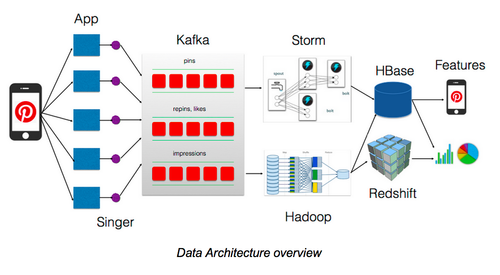
\includegraphics[width=1\textwidth]{pinterest_architecture.png}
	\caption{Schema - Architecture pinterest.com}
	\label{schema_pinterest_architecture}
\end{figure}
If you take a look at Figure \ref{schema_pinterest_architecture}, you can see a comparable data system architecture, implemented by pinterest.com\footnote{\cite{PINA}, Architecture of Giants: Data Stacks at Facebook, Netflix, Airbnb, and Pinterest}. Redis as a database on top of the hadoop cluster storage to serve for analytical purposes (e.g. ad serving of pinterest's adbuyers) or HBase on top of Hadoop cluster storage and Storm to serve features for the actual end-user of pinterest.com.\\

But we need to take care here: by creating new and more complex data systems from special purpose data systems, complexity is growing with it. How to ensure the system is avalaible with a reliable performance if something crashes? How to make sure data remains consistent and complete if things go wrong? How to scale the data system to be able to handle increased load?...\\
There are many apects which are crucial and influence the architecture of a data system like regulary constraints like data security, location of servers, SLA's\footnote{\cite{WKSLA}, \textit{Service Level Agreement, a commitment between a service provider and a client. Particular aspects of the service – quality, availability, responsibilities – are agreed between the service provider and the service user.}}\abk{SLA}{Service Level Agreement} or existing devlopment and operation skills - which very much depend on the specific situation.\\
Within the next chapters we will focus on the aspects which must be taken into account by any data system:

\begin{itemize}
			\item \nameref{tf_nfreq_scalability} (Chapter \ref{tf_nfreq_scalability}),
			\item \nameref{tf_nfreq_avrel} (Chapter \ref{tf_nfreq_avrel}),
			\item \nameref{tf_nfreq_maintainability} (Chapter \ref{tf_nfreq_maintainability}).\\
\end{itemize}

As many people and companies usually mess around with those terms, firstly we will develop a clear understanding on what they mean and later on take a closer look on how to apply algorithms, development and architectures to fulfill them appropriately.

\subsection{Scalability}
\label{tf_nfreq_scalability}
As is evident from the introduction of this chapter: the fact that a system is working reliable today doesn't mean it will necessarily work reliable in the future. The data system of ebay.com in 1999 was maxed out at handling \textbf{50.000} active listings\footnote{\cite{EBAYA}, slide 9}, imagine how the system would behave today at handling \textbf{1 billion} active listings\footnote{\cite{EBAYHP}}.
Obviously handling increased load (e.g. a larger amount of data needed to store or request to handle) is a major factor of a scalable data system.
\\[0.5 cm]
\hspace*{4mm}%
\fbox{%
  \hspace*{1.5mm}\hspace*{-1\fboxsep}%
  \parbox{0.08\textwidth + 5mm - 2\fboxsep}{%
\begin{minipage}{0.1\textwidth}
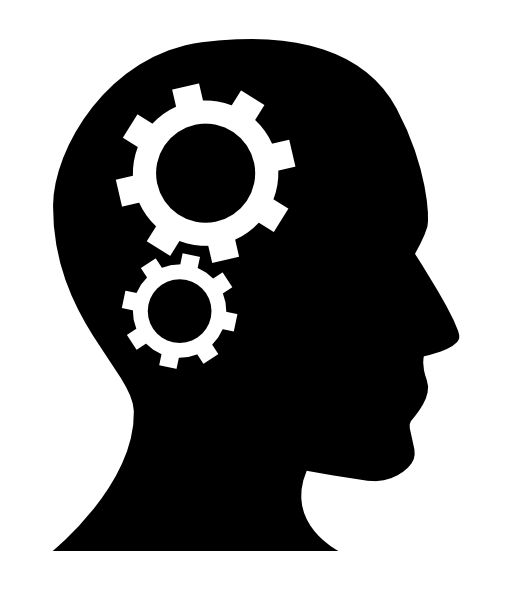
\includegraphics[width=\linewidth]{gear_brain.png}
\end{minipage}
  }%
}\hspace*{4mm}%
\begin{minipage}{0.8\textwidth}\raggedright
\textbf{Scalability} is the capability of data system to handle a growing amount of load (e.g. a larger amount of data needed to store or requests to handle). A data system is considered scalable if its capable of increasing it's total through-/output under an increased load when resources (typically hardware) are added. \\
\end{minipage}\\[0.4 cm]

Note that, ``\textit{scalability}'' isn't a binary tag that could be attached to a data system. It's pointless to say ``\textit{a data system is scalable}'' as well as ``\textit{a data system is not scalable}'', in either way you must think about ``\textit{If the load of a data system grows in a certain way, what are the options on the table for coping with the growth?}'' and ``\textit{How can we add ressources (hardware) to be able to handle the additional load?}''. \\
Therefore we will discuss the parameters and definition of \textbf{Load} (Section \ref{tf_nfreq_scalability_load}) and \textbf{Performance} (Section \ref{tf_nfreq_scalability_performance}) within the next section as well as \textbf{Approaches} for coping with load to achieve a certain performance (Section \ref{tf_nfreq_scalability_approaches}).

\subsubsection{Load}
\label{tf_nfreq_scalability_load}
To get an idea what \textit{load} of a data system actually means, how it could be described an measured, we will take a nother look at the example of ebay.com discussed so far. If we take a look back at the architecure of ebay at 1997-1999 (Figure \ref{schema_ebay_architecture_1997_1999} on page \pageref{schema_ebay_architecture_1997_1999}) we can already guess with increasing load (page requests to certain items listed on ebay.com and in this way calls to the database through the application) will reach its limit at the maximum amount of read requests the oracle database can serve. As the application tier (web server) has already been scaled horizontally to multiple nodes, the oracle database server reached its limit of physical growth in November 1999. \\
\begin{figure}[ht]
	\centering
  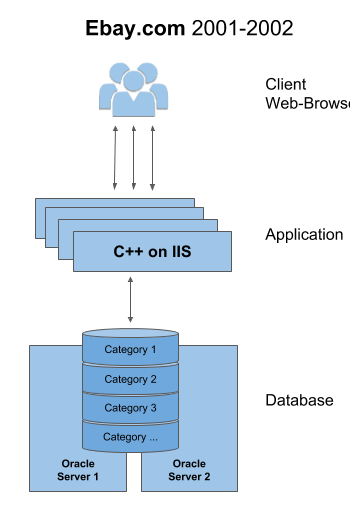
\includegraphics[width=0.4\textwidth]{Ebay_2002.png}
	\caption{Schema - Architecture Ebay.com April (2001 - December 2002)}
	\label{schema_ebay_2002}
\end{figure}

So ebay added an additional server to not just elmininate the SPOF\abk{SPOF}{Single Point Of Failure}\footnote{\cite{WPSPOF}, Single Point Of Failure} but to be able to failover but also they have splitted the database to be able to logically partition it into separate instances and in this way be able to scale horizontally. This was achieved in 2001 by splitting items by categories, as you can see in Figure \ref{schema_ebay_2002} on page \pageref{schema_ebay_2002}. In this simple way it was possible to distribute the load (mostly page requests for items) in an ``equal'' way to different physical nodes.
Later on they segmented whole databases into functional areas like hosts for item, user, account or transaction data as well as partitioned the data by typical usage characteristics to scale horizontally.\\

They obviously did furher optimizations at the whole data system to be able to cope with the increasing load, like disabling transactions, moving CPU-intensive\abk{CPU}{Central Processing Unit}\footnote{CPU, a processor or processing unit is an electronic circuit which performs operations on some external data source, usually memory or some other data stream is called central processing unit} work to the application tier (e.g. joins, referential integrity or sorting), extensive use of prepared statements...but as this techniques are not mainly specific for distributed systems and some of them not even recommened nowadays, we won't focuse on them within this lecture.\\

In the example of ebay.com, requests per item and category could be a valuable \textit{load parameter} for discussing scalability, since it determines the database requests per data record and partition - as proven by the the data system structure of ebay at 2002 as we see.
Your or other data systems you have seen so far most likely have very different characteristics, but you can apply similar principles to reason about their load.
\\[0.5 cm]
\hspace*{4mm}%
\fbox{%
  \hspace*{1.5mm}\hspace*{-1\fboxsep}%
  \parbox{0.08\textwidth + 5mm - 2\fboxsep}{%
\begin{minipage}{0.1\textwidth}
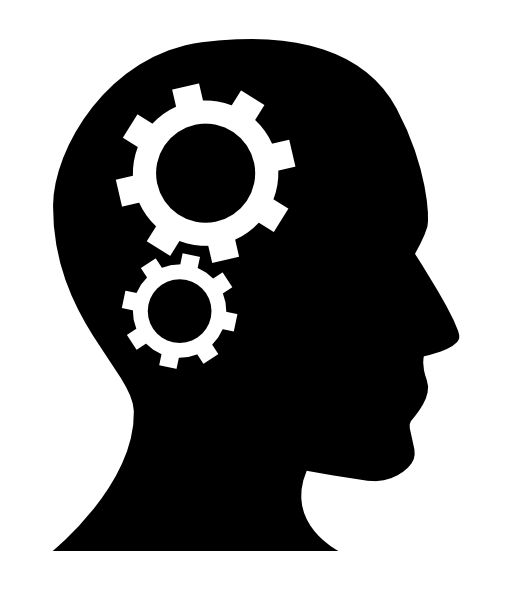
\includegraphics[width=\linewidth]{gear_brain.png}
\end{minipage}
  }%
}\hspace*{4mm}%
\begin{minipage}{0.8\textwidth}\raggedright
The \textbf{load} of a data system is a measurement of the amount of computational work it performs (depending on the architecture in-place), e.g. the number of (concurrent) reads from a data storage, writes to a data storage or the ratio between reads and writes. The maximum load is defined by the weakest part of the architecture (=\textit{bottleneck}). \\[0.4 cm]
\end{minipage}\\

\subsubsection{Performance}
\label{tf_nfreq_scalability_performance}
Now that we have described what \textit{load} of a data system means as well as what \textit{load parameters} could be, we will examine more closely what happens when the load increases. Usually there are two important cases you need to think about while developing data systems:\\
\begin{samepage}
\begin{itemize}
			\item The load parameter increases, but all ressources (e.g. number of server, CPU or memory) stay the same - how is the performance of the data system affected?
			\item The load parameter increases - how much do you need to increase the ressources (e.g. number of server, CPU or memory) to keep the performance stay the same?\\
\end{itemize}
\end{samepage}

But how to answer them? Therefore we need performance numbers. In case of data systems measurement, methods usually are \textbf{throughput} (number of records that can be handled), e.g.:
\begin{itemize}
			\item read/writes per second (in case of MongoDB up to 100.000 read/writes per second)
			\item messages processed (in case of Apache Kafka and Linkedin more than 2 million records per second on just 3 nodes)
			\item data processed (in case of Apache Hadoop and MapReduce terabytes of data within several seconds)\\
\end{itemize}

or if your buidling a data-system which works as the backend of a end-user facing application like a website, it's more about the \textbf{response time}, which means the time between sending a request and receiving the response. For instance if we think about the example of ebay.com within the previous chapters, as of 2012 they had 1 billion items accessible at any time, needed to serve 2 billion page requests each day and had to fulfill each of them within fractions of a second\footnote{\cite{EBAY2012}, https://hughewilliams.com/2012/06/26/the-size-scale-and-numbers-of-ebay-com/}. \\

Regardless of throughput or response time - if we think about performance we don't think about a single number, but a distribution of values that we can measure. If you will repeat the same page request, read or writes on the same data system: response time and throughput will inevitable vary somehow. There are simply too many factors you usually cannnot contain:
\begin{itemize}
			\item network issues (e.g. latency or TCP packet loss and retransmission)
			\item os issues (e.g. a page faults, context switches or running background processes)
			\item physical issues (e.g. a damaged disk/ssd or overheating of a CPU and, associated therwith a decreased processing power) \\
\end{itemize}

Therfore it is common to use an average for measuring throughput or response times. \textit{Average} doesn't refer to a particular formula, we will briefly discuss 3 that are commonly used:
\begin{itemize}
			\item \textbf{arithmetic mean}\footnote{Sum of values divided by the number of values.} (easy to calculate but ignores ratios and is highly affected by statistical outliers, so it cannot tell you how many requests, reador writes actually have had a worse performance)
			\item \textbf{median}\footnote{A median separates the higher half of values from the lower half.} (easy to calculate and less distorted by outliers)
			\item \textbf{percentiles}\footnote{A measure used for indicating a certain percentage of scores falls below that measure.} (easy to calculate, not distorted by outliers) \\
\end{itemize}

\begin{figure}[ht]
	\centering
  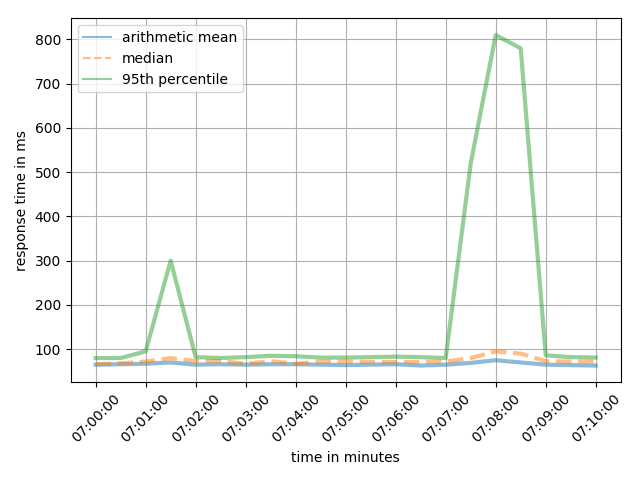
\includegraphics[width=1\textwidth]{mean_average_percentile_plot.png}
	\caption{Schema - Arithmetic Mean, Median and Percentiles - Example}
	\label{schema_mean_average_percentile_plot}
\end{figure}

As you can guess, evaluating symmetric distributions with no outliers, \textit{arithmetic mean} will be the best choice, but as we are looking at performance parameters like throughput and response times, symmetric distribution is a whishful thinking. More usually throughput and response times will result in skewed distributions, so \textit{median} seems to be the better choice, as it doesn't ignore ratio and outliers completely. For instance if you calculate the median for latency (y-axis) of reads in a given timeframe (x-axis) from a data system as illustrated in figure \ref{schema_mean_average_percentile_plot} on page \pageref{schema_mean_average_percentile_plot}. You can see a small peak at \textit{07:08:00} but it still looks fine as the median response time is < 100ms. But what about the green graph (\textit{95th percentile})? That's the main reason why using percentiles is pretty common, especially the 95th, 99th or 99.9th percentile (abbreviated \textit{p95}, \textit{p99}, \textit{p999}) is frequently used in SLA's\footnote{\cite{WKSLA}, \textit{Service Level Agreement, a commitment between a service provider and a client.}}. Percentiles define thresholds at which 95\%, 99\% or 99,9\% of requests, reads or writes are beneath that threshold. Looking back at figure \ref{schema_mean_average_percentile_plot} this would mean that 95\% of all requests, reads or writes done by user are faster or equal 810ms and 5\% will result in a response time > 810 ms, which in case of a customer facing data system could mean: 5\% unsatisfied users and in this way probably a loss of possible leads (e.g. purchases on a webshop or subscriptions for a video streaming platform) and ultimately loss of revenue.\\
So why don't use 99,9th percentile every time as it is the best? This is a major cost factor, optimizing the last percentiles gets really expensive, especially as this usually involves a lot of hardware redundancy as well as eliminating factors outside of your control. At a certain point costs will be bigger than the benefits, so you need to make a trade-off. \\[0.5 cm]
\hspace*{4mm}%
\fbox{%
  \hspace*{1.5mm}\hspace*{-1\fboxsep}%
  \parbox{0.08\textwidth + 5mm - 2\fboxsep}{%
\begin{minipage}{0.1\textwidth}
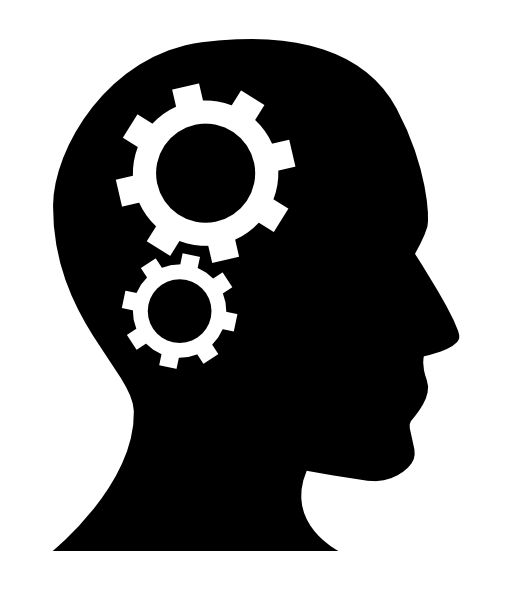
\includegraphics[width=\linewidth]{gear_brain.png}
\end{minipage}
  }%
}\hspace*{4mm}%
\begin{minipage}{0.8\textwidth}\raggedright
\textbf{Performance} of a data system is defined by system throughput and response time, e.g. number of transactions (like read/write operations), processed records (like aggregations for analytical purposes) or even system commands (like an \textit{update statistics} or rebalancing of several data nodes) under a given workload and for a specific timeframe. It usually depends on a variety of influencable as well as uninfluencable factors of the system itself, like network latency, a page fault or damaged disk. \\[0.4 cm]
\end{minipage}\\

\subsubsection{Approaches For Scaling}
\label{tf_nfreq_scalability_approaches}
Now that we are familiar with describing \textit{load} and measuring \textit{perfromance} we can answer the question: how to ensure performance, even if the load increases?
As we have seen by the example of ebay.com within the previous chapters, a system which is able to cope with a load, won't be able to handle 10 times of that load. This needs us to think about the architecture right at the beginning as well as each time the load significantly increases. As we have learned there are two ways to scale an architecture of a data-system:

\begin{itemize}
			\item \textbf{scale up/vertical} - replace a server by a more powerful one
			\item \textbf{scale out/horizontal} - distribute the load towards multiple server instead of one\\
\end{itemize}

A data-system running on a single server is easier to develop, as you can neglect a lot of factors that are specific to distributed systems (e.g. replication, partitioning or transactions and consistency across nodes), but more powerful machines are also more expensive and at a certain point you will reach the physical limit as ebay.com did. \\
A distributed data-system will require more development, test and operational effort as well as result in complexity but servers will be much cheaper as you make use of less powerful machines (\textit{``commodity'' hardware}) and you are able to bypass the inevitable physical limit of a single server. \\
In practise you won't choose one pattern only (scale up or out) as well-working architectures need a carefully chosen mixture of both approaches, e.g. it doesn't make sense to make use of a lot of poorly powered servers (like a Raspberry Pi) instead of some more powerful machines in terms of unnecessary costs, network and software complexity. As you may guess, there is no one-size-fits-all solution and architecture for scalabale data-systems as the requirements are highly specific to each data-system itself. The \textit{load parameter} may be strongly influenced by:

\begin{itemize}
			\item the \textbf{volume of data} to store
			\item the \textbf{number of read or write operations}
			\item the required \textbf{throughput} or \textbf{response time}
			\item the \textbf{structure of the data} and \textbf{how it's accessed} (e.g. relational, document-oriented, graph)
			\item and many more.\\
\end{itemize}

Right now it shall be sufficient that you know the basics concepts of scalability, later within this lecture, we will make use of it when looking at distributed data storage and processing as well as related software and frameworks. At the end you should be able to apply those concepts to any data-system and be able to make reasonable decisions in terms of scalability.

\newpage

\subsection{Reliability}
\label{tf_nfreq_avrel}
In general \textit{reliability} represents the probability that something/someone will perform a required function without failure under stated conditions for a period of time, e.g. a test will be reliable when it gives the same repeated result under the same conditions. \\Or more pragmatic: \textit{something works correctly even if things go wrong}.\\

So what are the \textit{faults}, mentioned in the previous defintions that we need to anticipate, about?

\subsubsection{Hardware Faults}
\label{tf_nfreq_reliability_hardware_faults}

Obviously any hardware produced has a certain lifespan, buth that's not the only reason for hardware faults. If you're talking with operators of data centers, they will provide you with a broad list of common as well ase spine-chilling causes for hardware faults as:\\

\begin{itemize}
			\item broken HDDs\abk{HDD}{Hard Disk Drive}\footnote{HDD, a hard disk drive is a non-volatile computer storage device containing magnetic disks or platters rotating at high speeds.} or SSDs\abk{SSD}{Solid-State Drive}\footnote{SSD, a solid-state drive is a nonvolatile storage device that stores persistent data on solid-state flash memory.}
			\item faulty RAM\abk{RAM}{Random Access Memory}\footnote{RAM, a Random Access Memory is the hardware in a computing device where the operating system, application programs and data in current use are kept so they can be quickly reached by the device's processor.} or CPUs\footnote{CPU, a processor or processing unit is an electronic circuit which performs operations on some external data source, usually memory or some other data stream is called central processing unit}
			\item broken power adapters, switches or whole network outages
			\item unplugged network cables or even connected to the wrong port
			\item and many many more.\\
\end{itemize}

As this seems pretty unlikely at first sight - it's definitely not. For instance let's have a look at hard drives, especially in distributed data-systems you will have a lot of them. If you think about Apache Hadoop, you usually use low-class server (\textit{``commodity'' hardware}), e.g. \textit{ProLiant DL380 Gen10 Server} as they provide a good ratio of:

\begin{itemize}
			\item computing power (CPU) / Storage (HDD), 
			\item rack space (2 RU\abk{RU}{Rack Unit}\footnote{\cite{WPRU}, Rack Unit is a unit of measure defined as 44.50 millimetres (1.75 in). It is most frequently used as a measurement of the overall height of rack frames.}) / storage and 
			\item benefit/cost.\\
\end{itemize}
Each of this servers can store 19 HDDs, if you build a hadoop cluster with those servers, e.g. with about 100 nodes, this means 1,900 HDDs. Based on a regularly study by BackBlaze\footnote{\cite{HDDSTDY}, https://www.backblaze.com/blog/hard-drive-failure-rates-q1-2017/} (a big data storage center provider like Amazon AWS) with a set of 82,516 HDDs, the average annual failure rate is about 2.11\%. Regarding our previous Hadoop example containing 1.900 HDDs, we can suppose that nearly any week a HDD will fail. If we would make use of the particular HDD model \textit{Seagate ST4000DX00} with a failure rate of 35,88\% (also mentioned within the study) this would mean nearly 2 HDDs would fail each day.\\

In single server data systems it is possible to mitigate those problems by adding redundancy to individual hardware parts to minimize the failure rate of the whole system to a point where a failure is very unlikely, as at any time a redundant part can take over. This could mean, dual power adapters (like used by the previous mentioned \textit{ProLiant DL380 Gen10 Server}), RAID\abk{RAID}{Redundant Array of Independent Disks}\footnote{RAID, is a data storage virtualization technology that combines multiple physical disk drive components into one or more logical units for the purposes of data redundancy, performance improvement, or both.} configurations or hot-swappable CPUs.
As data volumes and computing demand increases, data-systems need to be distributed among several servers, which proportionally increases the rate of hardware faults and system failures, like discussed above regarding HDD faults. Therefore distributed data systems need to be able to tolerate the loss of entire machines, requiring software to be fault-tolerance additionally to hardware redundancy. 
But those distributed data systems have further advantages, a system that tolerates failure of single machines can be restarted, patched, updated (\textit{rolling-upgrades}) or maintained - one node at a time - without a downtime of the whole data-system.

\subsubsection{Software Faults}
\label{tf_nfreq_reliability_software_faults}
When we talk about software faults in terms of distributed data-systems, we don't talk about usual bugs but rather faults which affect the whole data-system integrity and reliability. Such faults are harder to anticipate than usual bugs of single-server applications, as they usually tend to be caused by the environment (e.g. multiple servers, network, dependencies, special and unusual circumstances), are difficult to test, and are even worse in their result as they can cause a failure of the whole data-system.
Examples could be:
\begin{itemize}
			\item a runaway and/or zombie process that extensively used up some shared ressource (e.g. network, CPU, RAM, disk space)
			\item a software bug causing the whole cluster to fail (e.g. the Hadoop Ressource Manager YARN\abk{YARN}{Yet Another Resource Negotiator}\footnote{YARN, Yet Another Resource Negotiator} once had a bug\footnote{\cite{YARNKPBUG}, https://issues.apache.org/jira/browse/YARN-2809}, that if you removed a cgroup (\textit{control group}) under some circumstances (\textit{race conditions}) a kernel panic and in this way a failure of multiple server was caused
			\item a service the whole data-system depends on slows done, becomes unresponsive or fails
			\item cascading failures (e.g. one server of the data-system fails due to heavy network traffic, causing the other servers to take over, in this way increasing network traffic for them too and finally all server will fail)\\
\end{itemize}

As you can see, most of the reasons for software faults are caused by assumptions about the environment that may not be true at some time and at some special circumstances. To avoid suffering those issues you need to carefully think about assumptions and interactions within the distributed data-system, you will need a lot of measuring, monitoring and you will do a lot of analyzing of the system behaviour in any special circumstance as well as testing even with forcing some servers of the system to crash.

\subsubsection{Human Faults}
\label{tf_nfreq_reliability_human_faults}

We have been talking a lot about reliability so far, but what about the most unreliable factor: humans. We will briefly discuss some approaches to make a data-system reliable in terms of unreliable humans:
\begin{itemize}
			\item decouple places where people make the most failures from places they can cause failures, e.g. using production and development environments or providing interfaces or frameworks for an API instead of direct API access
			\item use extensive testing (e.g. unit test, system tests, integration tests) and automize them
			\item measuring and monitoring (e.g. performance metrics, error rates) allows to check wether assumptions or constraints are violated at an early stage \\[0.5 cm]
\end{itemize}

To sum up the last chapters: why do wee need reliability? Reliability is not just a major topic for stock exchanges, air line reservations or military. Failures of a data-system can cause data loss, lost productivity or sales loss and therefore huge costs and loss of revenue. There are special circumstances when you may choose to reduce reliability for the sake of time, development effort or operational costs (e.g. \textit{prototyping}), but you need to be very conscious and it's inevitable that at some point in the future you will need to invest the the saved effort, time and costs and probably a multiple of what it would have been before.\\[1.0 cm]
\hspace*{4mm}%
\fbox{%
  \hspace*{1.5mm}\hspace*{-1\fboxsep}%
  \parbox{0.08\textwidth + 5mm - 2\fboxsep}{%
\begin{minipage}{0.1\textwidth}
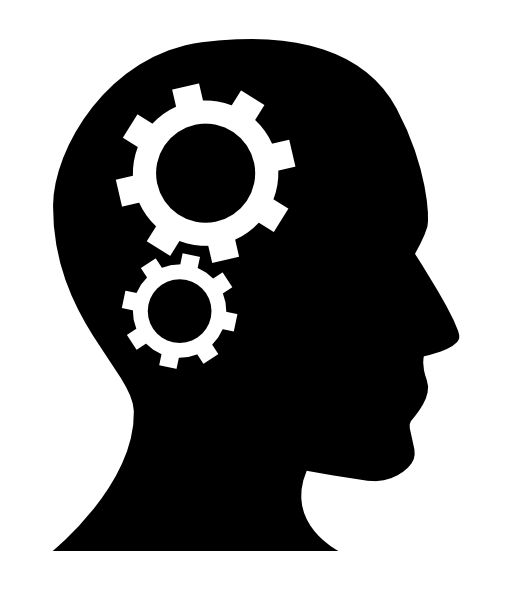
\includegraphics[width=\linewidth]{gear_brain.png}
\end{minipage}
  }%
}\hspace*{4mm}%
\begin{minipage}{0.8\textwidth}\raggedright
\textbf{Reliability} in terms of hardware, software or especially data-systems can be defined as the ability of a system to function as specified and expected. A reliable data-system also detects and tolerates faults due to mistakes of users, hardware or lower parts of the data-system itself as well as ensures the required performance under any expected load. \\[0.4 cm]
\end{minipage}\\

\subsection{Maintainability}
\label{tf_nfreq_maintainability}
Maintenance is known as one of the biggest costs at software devlopment and in the same way a very unfamous topic to software engineers. Keeping a system running, investigating failures, fixing bugs, adding new features, adapting it to updates of underlying hard- and software - to name some usual tasks.\\

A data-system should be designe to minimize effort during maintenance and in this way making it more reliable. We will briefly discuss 3 major topics: \textit{operability}, \textit{simplicity} and \textit{evolvability}.

\subsubsection{Operability}
\label{tf_nfreq_maintainability_operability}
The main goal of operability should be to make operations easy to keep the system running smoothly, this means making routine tasks easy and enable operations ressources to use their time for important tasks. This can be achieved by:
\begin{itemize}
			\item good documentation and operational model (a data-system which can be understand easily can be operated more easily)
			\item transparency (visibility into the data system and runtime behaviour, e.g. by log files or monitoring tools)
			\item no dependencies between single services or server (allow single server to go down for maintenance tasks, e.g. patches, update or restarts)
			\item self-healing if possible, but also possibilities to override for operators\\[0.5 cm]
\end{itemize}

\subsubsection{Simplicity}
\label{tf_nfreq_maintainability_simplicity}
When you start a development project everything is pretty simple and probably well-documented but later on with multiple developers, features, services and servers, it gets more complex, hard to understand by a developer and especially more difficult to handle by administrators. As a lot of issues caused by this are not specific to data-systems we will focuse on complexity and abstraction, as reducing complexity should be the main goal when devloping distributed data-systems. Making a system less complex doesn't require reducing functionaility, it's more about removing unnecessary complexity.\\
For instance if your data-system is crunching a lot of data for a very plain purpose, like parsing web server log files for analytical purpose to get to know how many people have visited your website - you could do this counting in Java (MapReduce) but this will probably be about 50 lines of code, a lot of libraries, testing and dependencies - making operations more difficult in the same way. If you would do this using Hive on HDFS your done with a one-line SQL statement.\\

However finding useful abstractions is not that easy and needs a lot of experience, but when you are developing something you should always ask yourself: do I make use of abstraction and will the complexity be at a manageable level?


\newpage
\section{Storage Concepts}
\label{tf_storageconcepts}
to-be-added

\newpage

\section{Data Models And Access}
\label{tf_dma}
Data Models are one of the most crucial part of any data-system as they significantly influence actually everything: development and required skills, operations, backends and frontends as well. \\
For instance, if you choose a document oriented data store (e.g. MongoDB) to serve a web-based application, as it is pretty easy to build a REST API on top of it and JSON data and JavaScript Frontends (e.g. based on AngularJS) are a perfect match but don't think about how the data will be queried later - you may run into a lot of trouble. For example if your data consist of many business objects which are highly complementary and the frontend usually needs multiple business objects within one request, you're probably out of luck as document-oriented storages perform pretty well when only reading from one collection but not at joining them. You could probably put all related business objects in one document, but as this is unnecesessarily redundant it will burst your data storage very soon. \\
To conclude: there are many different kinds of data models and every data model has it strengths but weaknesses as well. Some are easy to use - some not, some operations using them will be fast - others definitely not, some are very storage efficient - some note... As you can see it's not that easy to decide which data model to use as it has a profound effects on the whole data-system you are building, even that far that a wrong decision could be a show stopper at some time in development.\\
It needs a lot of experience and very forward-looking to choose a data model that fits best to your data-system. Within the next chapters we will talk about the most common data models (\textit{relational}, \textit{document-oriented}, \textit{graph}), how to access them {\textit{SQL}, \textit{MapReduce}, \textit{SPARQL}), how they differ, advantages and disadvantages. \\
At the end you should have a basic understanding on how they work and which of them fits best to a certain problem.

\subsection{Data Models}
\label{tf_dma_datamodels}

\subsubsection{Relational Data Model}
\label{tf_dma_datamodels_rdm}

Firstoff we will take a look at the relational data model, originally introduced by Edgar Frank Codd in 1970\footnote{\cite{CODDRDM}, `A Relational Model of Data for Large Shared Data Banks'' - IBM Research Laboratory, San Jose, California}. \\[0.5 cm]
\hspace*{4mm}%
\fbox{%
  \hspace*{1.5mm}\hspace*{-1\fboxsep}%
  \parbox{0.08\textwidth + 5mm - 2\fboxsep}{%
\begin{minipage}{0.1\textwidth}
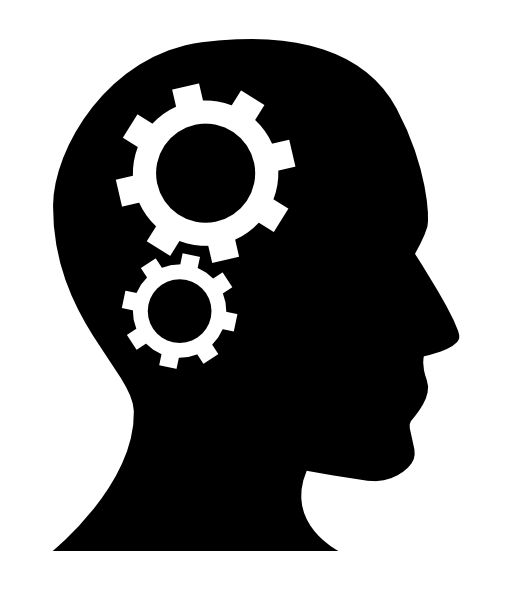
\includegraphics[width=\linewidth]{gear_brain.png}
\end{minipage}
  }%
}\hspace*{4mm}%
\begin{minipage}{0.8\textwidth}\raggedright
The \textbf{relational model} is an approach to managing data using a structure and language consistent with first-order predicate logic where all data is represented in terms of tuples and grouped into relations. 
\end{minipage}\\[0.5 cm]

Having its roots in the 1970's the relational data model had the idea to hide implementation details (e.g. internal representation of data in a data store) from developers by providing a cleaner, \textit{declarative} and \textit{read-on-schema} interface for specifying data and querying it. Developers can state what information the database contains and what information they want from it - the database itself will take care of describing, storing and retrieving data for developers. As you have already learned the basic about relational databases, indices, concepts like normalization and much more we will take a quick look at an example and afterwards conclude about advantages and disadvantages compared to other data models. \\

Let's take a look at figure \ref{schema_facebook_relational_model} on page \pageref{schema_facebook_relational_model} as an example. Here you can see how a Facebook profile could be represented in a very simple (and not fully normalized) relational data model. 
The table \lstinline{user} works as the main entity, as it's the profile page of a user. As a user is unique we also have a unique identifier (\lstinline{id}) as well as some information regarding the user within the same table (e.g. \lstinline{first} and \lstinline{last_name} or who they are \lstinline{married_to}). 
People may have worked for different companies (table \lstinline{companies}), lived in several cities {table \lstinline{cities}} or visited more than one university (table \lstinline{universities}) so we put that into separate tables including a foreign key (\lstinline{user_id}) of the referring table {\lstinline{user}}.\\

\begin{figure}[ht]
	\centering
  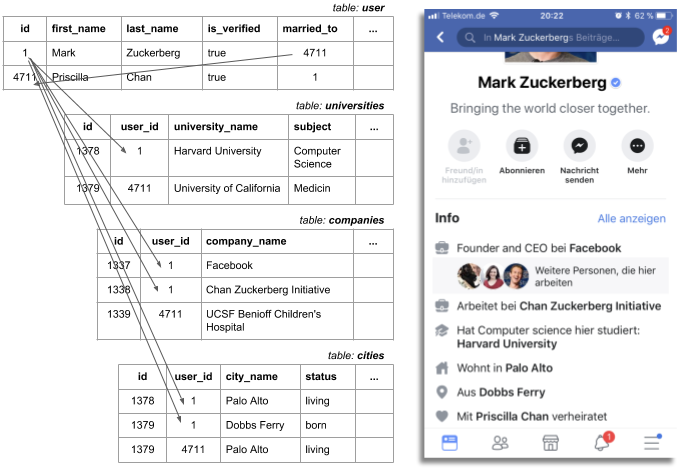
\includegraphics[width=1\textwidth]{relational_model_zuckerberg.png}
	\caption{Schema - Facebook Profile - As Relational Model}
	\label{schema_facebook_relational_model}
\end{figure}

\newpage

Relations are represented by \textit{tables} and tuples are represented by \textit{rows}. Rows can easily be inserted or fetched all-at-once, by using an id or a \textit{primary}/\textit{foreign key} unlike \textit{document-oriented} data models, where you:
\begin{itemize}
			\item sometimes need to make use of access paths,
			\item need to think about nested structures,
			\item need to worry about unknown fields as those systems are usually \textit{schema-on-read} or 
			\item or intensively need to think about possible performance issues and how the system will probably execute your query as the execution engine is usually not that mature as the one of a relational system,
			\item it's more difficult to understand how the systems works, as sometimes you don't even have a query-explain feature like in relational databases, so you won't be able to investigate or guess in advance how it will behave in detail during execution.\\ 
\end{itemize}
But as relational data models are also mostly used by applications, we need to talk about a frequently discussed issue: \textit{object-orientation}. As applications are \textit{object-oriented} you need to make use of a translation layer between an applications and relational model to enable the applications to make use of the data. There are many frameworks available to serve this translation called ORM\abk{ORM}{Object-Relational-Mapper}\footnote{ORM, Object-relational mapping is a programming technique for converting data between incompatible type systems using object-oriented programming languages.}, e.g. Hibernate\footnote{\cite{ORMHBN}, http://hibernate.org/} in case of Java or SQLAlchemy\footnote{\cite{ORMSQLAL}, https://www.sqlalchemy.org/} in case of Python to name only 2 of them. Those frameworks will require additional code, skill and development time, as systems using the document-oriented model are regularly used without additional frameworks for data translation, e.g. an AngularJS application using MongoDB. \\
But systems using a relational model are mostly more resilient as they usually gained several years or even decades of research, experience and development time, while document-oriented that are still widely used today just started in the early 2000's.\\
For instance many of them have highly sophisticated query optimizer which automatically decide which part of the query needs to be executed when, in which order and which index {e.g. \lstinline{user_id} of the previous example} is probably the best one to use - most of the document-oriented systems don't even have something that is worth to be called a query optimizer as their capabilities are far behind the relational ones. \\
But that's also due to the fact that relational and document-oriented data models are completely different in terms of relationship implementation: both of them are able to represent \textit{many-to-one} or \textit{many-to-many} relations but in a different manner. \\
Relational data models make use of \textit{primary} and \textit{foreign keys} which can easily be used for indices, document-oriented data models need to make use of nested structures (most commonly used) or \textit{document references} and joins to other collections (e.g. \lstinline{\$lookup} in MongoDB\footnote{\cite{MDBLKP}, https://docs.mongodb.com/manual/reference/operator/aggregation/lookup/}, \lstinline{populate()} in Mongoose\footnote{\cite{MGPPL}, http://mongoosejs.com/docs/populate.html} or Joins in RethinkDB\footnote{\cite{RDBJN}, https://www.rethinkdb.com/docs/table-joins/}) - both of them are resulting in expensive IO and CPU operations as either you need to make use of features that are extremely immature compared to their relational counterpart or the whole document needs to be read, which can also be very wasteful on large documents. \

This behaviour of document-oriented systems also applie for writes, as they usually require to rewrite the whole document in document-oriented data-systems. 
But to be fair, most document-oriented systems weren't initially designed with serving relationale dependencies or querying in mind, but rather for the sake and benefits of: 
\begin{samepage}
\begin{itemize}
		\item being object oriented, 
		\item easy to be altered, 
		\item  being semi-/unstructured and schema-``free''.\\
\end{itemize}
\end{samepage}
An in this way being the whole opposite of the relational data model.


\subsubsection{NoSQL Data Model}
\label{tf_dma_datamodels_dodm}

As we have discussed the relational data model in the previous chapter we will now take a closer look on non-relational data models, probably known as \textit{NoSQL}. \\
Even due to the fact that there have been some approaches and databases in the past (back to 1960's), the term \textit{NoSQL} and data-systems using it, gained their popularity in the early twenty-first century. The NoSQL wave was initially triggered by the emerging wave of \textit{Web 2.0} companies like Facebook, Google or Amazon, whose data-systems needed to cope with data sizes, throughput, response times and the need of high scalabilty, which could not be handled by using traditional relational data-systems anymore\footnote{\cite{IBMNS}}. Beside that the limitations of the relational data model for \textit{Web 2.0} kind of data, probably was on of the biggest issue, log files and textual data of social media websites or e-commerce shops are not very structured and even if they were, they probably changed their structure very frequently over time. \\
NoSQL data-systems like HBase, BigTable or Cassandra emerged by those needs, e.g.:
\begin{samepage}
\begin{itemize}
\item \textbf{Cassandra}, initially developed by Avinash Lakshman and Prashant Malik (Facebook employees) because of the need to solve the inbox search problem of the Facebook messenger\footnote{\cite{FBISP}, https://www.facebook.com/note.php?note\_id=24413138919} and later on released to be \textit{OpenSource} in 2008 or 
\item \textbf{BigTable}, initially developed by Google in 2004 to support several data intensive applications of google, such as web-indexing, GoogleMaps or GoogleMail and later on released as a public service in 2015\footnote{\cite{BTREL}, https://cloud.google.com/bigtable/docs/release-notes}.\\
\end{itemize}
\end{samepage}

As you can see NoSQL data-systems are increasingly used by BigData and real-time web and analytical applications as they can cope better with frequently changing data structures and are easier to scale horizontally, compared to their relational counterpart.\\

NoSQL data-systems are somethimes also called \textit{``Not only SQL''} to emphasize that they may support SQL-like query languages, even if their storage engine has ``nothing'' in common with traditional relational data-systems, e.g.:\\
\begin{samepage}
\begin{itemize}
\item \textbf{Hive}, initially developed by Facebook, is an abstraction layer to access data on a distributed file system (e.g. Hadoop HDFS or Amazon S3) without the need of programming MapReduce jobs by using SQL-like queries (\textit{HiveQL\footnote{\cite{AHW}, https://hive.apache.org/}}) and \textit{schema-on-read} or 
\item \textbf{Cassandra}, initially developed by Facebook as a NoSQL distributed key-value data store, which also provides a SQL-like query language, called \textit{CQL}\footnote{\cite{CQL}, http://cassandra.apache.org/doc/latest/cql/}.\\[0.5 cm]
\end{itemize}
\end{samepage}


\hspace*{4mm}%
\fbox{%
  \hspace*{1.5mm}\hspace*{-1\fboxsep}%
  \parbox{0.08\textwidth + 5mm - 2\fboxsep}{%
\begin{minipage}{0.1\textwidth}
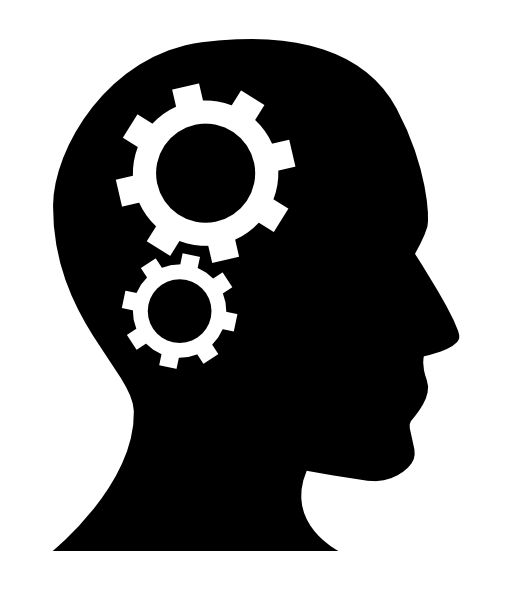
\includegraphics[width=\linewidth]{gear_brain.png}
\end{minipage}
  }%
}\hspace*{4mm}%
\begin{minipage}{0.8\textwidth}\raggedright
\textbf{NoSQL} in terms of BigData, is a theorem for managing data using document-oriented, key-value or graph structures, where all data is represented in terms of documents, key-value pairs, graphs (nodes, edges, properties) or mixed approaches.
\end{minipage}\\[0.5 cm]

Let's take a another look at the example in Figure \ref{schema_facebook_document_oriented_model} on page \pageref{schema_facebook_document_oriented_model}, which we already discussed by regards of the relational data model in chapter \textit{\ref{tf_dma_datamodels_rdm} \nameref{tf_dma_datamodels_rdm}}. Here you can see how the same Facebook profile could be represented in a very simple document-oriented data model (e.g. \textit{JSON}\abk{JSON}{JavaScript Object Notation}\footnote{\cite{JSONW}, JSON (JavaScript Object Notation), a lightweight data-interchange format, easy for humans to read/write and machines to parse/generate.}). Representing a data structure like a (Facebook) profile, which is mostly a self-contained document, using JSON could be vary appropriate. As you can see in this case the document structure has a better \textit{locality} than the relational structure, where you would need to fetch rows from multiple tables and join them. Using the document-oriented structure, you just need to fetch one document as all the information you need to create the profile page, are at one place. The document-oriented structure allows you to easily access previously \textit{normalized} data (\textit{one-to-many relationship}), like \lstinline{companies} a person worked for or \lstinline{cities} a person lived in, just by it's explicit tree structure.\\

\begin{figure}[ht]
	\centering
  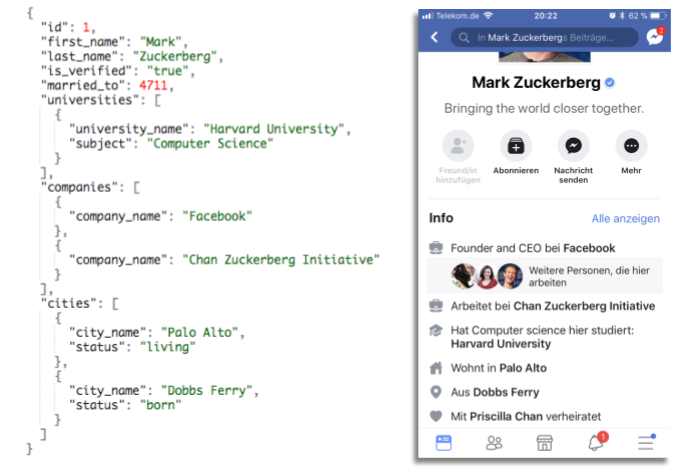
\includegraphics[width=1\textwidth]{document_oriented_data_model_zuckerberg.png}
	\caption{Schema - Facebook Profile - As Document Oriented Model}
	\label{schema_facebook_document_oriented_model}
\end{figure}

Let's have a closer look on 3 topics often discusses as advantages of the document-oriented data model:

\subsubsubsection{Schema Flexibility}
Most document-oriented data-systems do not enforce a defined schema unlike the relational data model. For instance if we take look at Figure \ref{schema_facebook_document_oriented_model} arbitrary keys and values, e.g. additional information like interests or favourite movies could be added to the document without causing any issues. But if your reading documents later on, you have no guarantee wether a certain document contains a required field or not, instead you need to be sure or make use of additional operators, for instance the \lstinline{$exists} operator in case of MongoDB to check wether a required field exists or not\footnote{\cite{MDBEX}, https://docs.mongodb.com/manual/reference/operator/query/exists/}. \\
NoSQL data-systems are often called \textit{schemaless}, which is wrong, as the engine which is processing the data usually assumes some kind of structure. This is called \textit{schema-on-read}, the structure of the data is implicit and only interpreted when the data is read, whereas traditional relational data-systems are \textit{schema-on-write} and explicit forcing the engine to ensure all data which will be written is conform to the schema. This approach is very valuable in case an application wants to change the format of it's data on a regular base. In case of a relational data-system you would need to run an \lstinline{ALTER TABLE} or even \lstinline{CREATE TABLE} statement, which are highly IO and CPU intensive operations. As a very drastic example, if you run an \lstinline{ALTER TABLE} statement in MySQL, this will not only cause a lock for \lstinline{INSERT} and \lstinline{UPDATE} statements on the same table (if not using InnoDB), but also copying the entire table, which could take even hours depending on the size of the table\footnote{\cite{MYSQLAT}, https://dev.mysql.com/doc/refman/5.5/en/alter-table.html}.\\
To sum up, in case the data your data-system needs to store is heterogenous, whereby not all records share the exact same structure and/or the schema will frequently change for a subset or all of the data, \textit{schema-on-read} is an appropriate approach.

\subsubsubsection{Data Locality}
As \textit{schema-on-read} data is usually represented (\textit{encoded}) as a single document (e.g. JSON or CSV\abk{CSV}{Comma-Separated Values file}\footnote{CSV, a text file that uses a comma to separate values}) or as their binary/serialized counterpart (e.g. Avro\footnote{\cite{AVRO}, https://avro.apache.org/} or ORC\footnote{\cite{ORC}, https://orc.apache.org/}) and your application often needs to access the entire or a large part of the document, there is a huge performance advantage in terms of \textit{storage locality} compared to relational data models, which need to read and join multiple tables (e.g. compare Figure \ref{schema_facebook_relational_model} on page \pageref{schema_facebook_relational_model}) requiring probably more IO (e.g. disk seeks and reads) and CPU time (e.g. join operation).
But this could also be a pitfall, the advantage only applies if you need a large part of the required document at the same time, as the data-system usually needs to load the whole document, even if you only need one value, which could be vary expensive on large documents. 
Another disadvantage are updates, as the data-system usually needs to rewrite the whole document, even if you only change one value. As an example, if you update a field in MongoDB, e.g. incrementing a counter:
\begin{lstlisting}[language=bash,frame=none,numbers=none,xleftmargin=0.05\textwidth,xrightmargin=0.05\textwidth]
 db.some_collection.update( { _id : ... }, { $inc : { y : 2 } } );
\end{lstlisting}
MongoDB is even that optimized, that no rewrite of the whole document is caused. But if you add another field, which causes the document to increase in size, it will no longer fit into the previously allocated space, the whole document needs to be rewritten anyway\footnote{\cite{MDBIP}, https://www.mongodb.com/blog/post/fast-updates-with-mongodb-update-in-place}.

\subsubsubsection{Application Code Simplicity}
Building a data-driven application obviously requires development and therefore application code that handles all interaction with the used data-system. Using a document-oriented data-system, where typically entire documents are loaded and written, usually requires less code within the application itself compared to relational data-systems where several tables need to queried, joined or updated at the same time. But in the same way it's a significant disadvantage of document-oriented data-systems, for instance if you would like to access a nested item within a document, or even the n-th tuple within the nested item, it often requires more code than an appropriate SQL would need. 
On the other way, just querying one single relational table requires way more code than querying one document, as the relational data model is not a natural fit to the world of object oriented programming languages. You need to write a lot of mappings to map the data to your application objects or use an ORM framework (as previously discusses) which also adds a lot of additional code in terms of libraries to your application. The document-oriented data model is a much more natural fit to objects uses in object-oriented programming languages and require less code to be linked to an objects, especially in the environment of data-intensive web applications, which for instance frequently make use JSON.
But there are also cases like \textit{many-to-many} relationships where a document-oriented data model will force you to write a lot of code. As we already discussed, document-oriented data-systems usually suffer and performing joins between different collections/entities, it's possible to reduce the need for joins by strictly denormalizing data - suffering all the disadvantages we have already discussed - or by moving the join operation from the data-system to the application code. This will in some way speed things up, but in the other way slow things down, as the application usually will not be as fast as a join within a database. This will also cause additional load on the application side as well as more complexity within the application code itself, as it needs to take care about everything the data-system would usually do.\\

There is no universal answer to the question which data model leads to more or less application code, as it highly dependends on the data itself, kinds of relationships, how the data is usually queried, which operations need to be run on the data-system and many more factors.


\subsubsection{Graph Data Model}
\label{tf_dma_datamodels_gdm}
to-be-added
\newpage
\subsection{Data Access}
\label{tf_dma_dataaccess}

\subsubsection{SQL}
\label{tf_dma_dataaccess_sql}

Let's take a look at SQL\abk{SQL}{Structured Query Language}\footnote{SQL, Structured Query Language}, originally introduced as ``SEQUEL'' by Donald D. Chamberlin and Raymond F. Boyce in 1974\footnote{\cite{SQLIBM}, ``SEQUEL: A STRUCTURED QUERY LANGUAGE'' - IBM Research Laboratory, San Jose, California} and inspired by Edgar Frank Codd's relational data model in 1970\footnote{\cite{CODDRDM}, `A Relational Model of Data for Large Shared Data Banks'' - IBM Research Laboratory, San Jose, California}. Despite not entirely adhering to the relational model as described by Codd, it became the most widely used database language and even supported in a limited way by NoSQL data-systems like Cassandra (\textit{CQL}\footnote{\cite{CQL}, http://cassandra.apache.org/doc/latest/cql/}) or Hadoop (\textit{HiveQL\footnote{\cite{AHW}, https://hive.apache.org/}}).
Designed for handling structured data and making it easily accessible to users and application code, it quickly became standard (ANSI 1986, ISO 1987). It obviously has been revised several times since then, to include a larger set of features but it's still used by an kind of relational data-system. Despite the fact that most SQL code is not completely portable among different, especially commercial, relational data-systems.\\
SQL is a set-based and declarative programming language unlike imperative or mixed-up programming languages, paradigms or approaches for accessing data (e.g. MapReduce, Spark). An imperative programming language forces the data-system to perform certain operation in a certain order. Imagine any application code you have written so far, for instance in Java, C++ or Python, the code will be executed line by line, doing some calculations, evaluating conditions and probably looping around several times. A declarative language like SQL (or programming languages like \textit{Prolog} or \textit{Lisp}, or even build languages like \textit{make}/\textit{cmake}) is usually more easy to work with than an imperative language. In case of SQL it is due to the fact, that it hides implementation details of the data-system, you usually do not need to think a lot about how the data is stored or retrieved as the data-system will take care about this as well as doing it with the best performance possible (\textit{query optimizer}).
Declarative languages are also easier to parallize in terms of horizontal scalability, as they only specify the pattern of the result, not the algorithm used to get the result. Whereas imperative programming languages and approaches are way more complicated to parallelize across multiple CPUs or nodes. As they require a lot of effort and attention, as imperative code specifies operations that need to happen in a specific order, need to be kept in-sync, are dependent of the results of previous steps and much more.\\


\subsubsection{MapReduce}
\label{tf_dma_dataaccess_mr}
\textit{MapReduce} is a programming paradigm and an associated implementation for processing and generating large data sets in parallel and distributed on a cluster, originally introduced by Jeffrey Dean and Sanjay Ghemawat (Google Inc.) in 2004\footnote{\cite{GOOMR}, ``MapReduce: Simplified Data Processing on Large Clusters'' - Google Inc.}. MapReduce is neither a declarative language nor a an imperative programming language, it's something in between - the logic of data querying is expressed with snippets of code, which are executed repeatedly by the processing framework/runtime system. 
The paradigm is based on specifying a \textit{map} function, which performs filtering and sorting, resulting in an intermediate set of key/value pairs and a \textit{reduce} function that merges all intermediate values associated with the same key (e.g. sum all values).
Applications written in this paradigm are automatically parallized and executed on several nodes of a cluster. The runtime system (e.g. YARN\footnote{\cite{YARNPP}, ``Apache Hadoop YARN: Yet Another Resource Negotiator'' - The Hong Kong University Of Science And Technology} in case of Hadoop) takes care of: 
\begin{samepage}
\begin{itemize}
\item the details of providing and partitioning the input data, 
\item scheduling the application code execution across all cluster nodes, 
\item saving intermediate states,
\item handling node failures,
\item inter-node communication and much more.\\
\end{itemize}
\end{samepage}
This enables programmers, without any experience with parallel or distributed systems, at a minimum effort, to easily utilize the computing ressources of distributed data-system and build data-driven applications that are highly scalable. \\

\begin{lstlisting}[aboveskip=1ex, belowskip=1ex, xleftmargin=18pt, emphstyle=\underbar, breaklines=true, showstringspaces=false, captionpos=b, caption=MapReduce Example - \textit{Word Count}, label=min_mapreduce, float,language=java]
map(String key, String value):
	// key: document name
	// value: document content
	for each word w in value:
		EmitIntermediate(w, 1);

reduce(String key, Iterator values):
	// key: a word
	// values: a list of counts
	int result = 0;
	for each v in values:
		result += v;
	Emit(key, result);
\end{lstlisting}

Above you can see a very simple pseudo code example (Code Snippet \ref{min_mapreduce}) to count the occurences of single words within a document (which is almost impossible to do in a SQL query on a database). The \lstinline{map} function is called once for each document and emits each word within it. The \lstinline{reduce} function sums together all counts emitted for a particular word. \\
The \lstinline{map} and \lstinline{reduce} functions are both defined with respect to data structured in \textit{key}/\textit{value} pairs. The \lstinline{map} function takes one pair of data with a type in one data domain, and returns a list of pairs in a different domain:\\
\centerline{\textit{map(k1,v1)} \ensuremath{\rightarrow} \textit{list(k2, v2)}}
This produces a list of pairs (keyed by \lstinline{k2}) for each call. After that, the MapReduce framework collects all pairs with the same key (\lstinline{k2}) from all lists and groups them together, creating one group for each key. The \lstinline{reduce} function runs in parallel for each group, which in turn produces a collection of values (\lstinline{v3}) to an associated key (\lstinline{k2}) within the same domain:\\
\centerline{\textit{reduce(k2, list(v2))} \ensuremath{\rightarrow} \textit{list(k2, v3)}}

The returns of all \lstinline{reduce} processes are collected as the desired result list. 
\newpage
Let's take a deeper look at the previous example and how the paradigm would work in detail, given the documents below:\\

\begin{lstlisting}[aboveskip=1ex, belowskip=3ex, xleftmargin=18pt, emphstyle=\underbar, breaklines=true, showstringspaces=false, captionpos=b, caption=MR Example - \textit{Word Count (Input Documents)}, label=min_mapreduce_documents,language=java]
document1 = "Da steh ich nun, ich armer Tor!";
document2 = "Und bin so klug als wie zuvor;";
document3 = "Heiße Magister, heiße Doktor gar";
document4 = "Und ziehe schon an die zehen Jahr";
document5 = "Herauf, herab und quer und krumm":
document6 = "Meine Schüler an der Nase herum.";
\end{lstlisting}

Which would result into 6 processes executing the \lstinline{map} function (special characters removed ahead as well as converting everything to lower-case to avoid duplicates):\\

\begin{lstlisting}[aboveskip=1ex, belowskip=3ex, xleftmargin=18pt, emphstyle=\underbar, breaklines=true, showstringspaces=false, captionpos=b, caption=MR Example - \textit{Word Count (\lstinline{map()} Calls)}, label=min_mapreduce_documents,language=java]
map(document1, "da steh ich nun ich armer tor");
map(document2, "und bin so klug als wie zuvor");
map(document3, "heiße magister heiße doktor gar");
map(document4, "und ziehe schon an die zehen jahr");
map(document5, "herauf, herab und quer und krumm");
map(document6, "meine schüler an der nase herum");
\end{lstlisting}

Creating the following partial results:\\

\begin{lstlisting}[aboveskip=1ex, belowskip=3ex, xleftmargin=18pt, emphstyle=\underbar, breaklines=true, showstringspaces=false, captionpos=b, caption=MR Example - \textit{Word Count (Partial \lstinline{map()} Results)}, label=min_mapreduce_documents,language=java]
p1 = [	("da",1), ("steh",1), ("ich",1), ("nun",1), ("ich",1), 
				("armer",1), ("tor",1) ];
p2 = [ ("und",1), ("bin",1), ("so",1), ("klug",1), ("als",1), 
				("wie",1), ("zuvor",1) ];
...
p6 = [	("meine",1), ("schüler",1), ("an",1), ("der",1), ("nase",1), 
				("herum",1)];
\end{lstlisting}

Those partial results calculated by the \lstinline{map} processes will be collected (if they have the same key/word) and handled over to the \lstinline{reduce} processes, which summarize the partial results:\\

\begin{lstlisting}[aboveskip=1ex, belowskip=3ex, xleftmargin=18pt, emphstyle=\underbar, breaklines=true, showstringspaces=false, captionpos=b, caption=MR Example - \textit{Word Count (\lstinline{reduce()} Calls)}, label=min_mapreduce_documents,language=java]
reduce("da", [1]); // = ("da", 1)
reduce("ich", [1,1]); // = ("ich", 2)
reduce("und", [1,1,1,1]); // = ("und", 4)
...
\end{lstlisting}

At the end, the desired output could look like:\\

\begin{lstlisting}[aboveskip=1ex, belowskip=3ex, xleftmargin=18pt, emphstyle=\underbar, breaklines=true, showstringspaces=false, captionpos=b, caption=MR Example - \textit{Word Count (Final Result)}, label=min_mapreduce_documents,language=java]
result = [ ("und", 4), ("ich",2), ("heiße",2), ("an", 2), ("da",1), 
		("steh",1), ("nun",1), ("armer",1), ("tor",1), ("bin",1), ("so",1), 
		("klug",1). ("als",1), ("wie",1), ("zuvor",1), ("magister",1), 
		("doktor",1), ("gar",1), ("ziehe",1), ("schon",1), ("die",1), 
		("zehen",1), ("jahr",1), ("herauf",1), ("herab",1), ("quer",1), 
		("krumm",1), ("meine",1), ("schüler",1), ("der",1), ("nase",1), 
		("herum",1) ]
\end{lstlisting}

Now that we know how \textit{Map} and \textit{Reduce} work in Detail, let's have a look at the whole process using the previous example. 

\begin{figure}[ht]
	\centering
  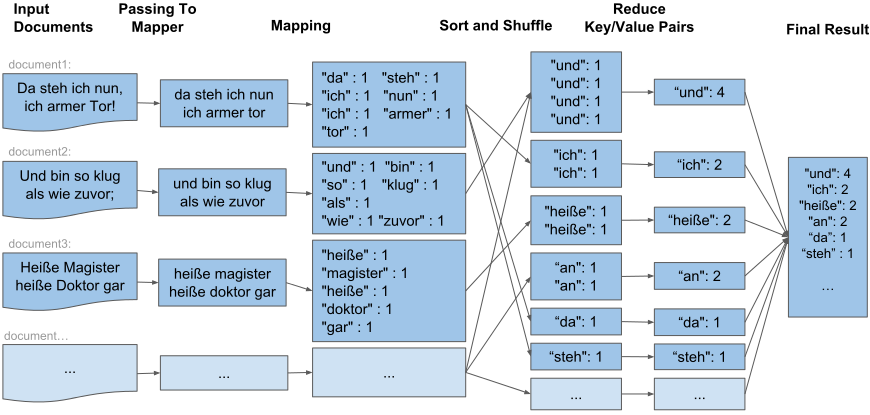
\includegraphics[width=1\textwidth]{map_reduce_phases_schema.png}
	\caption{Schema - MapReduce Phases - Word Count Example}
	\label{schema_map_reduce_phases_wordcount}
\end{figure}

Figure \ref{schema_map_reduce_phases_wordcount} on page \pageref{schema_map_reduce_phases_wordcount} illustrates the whole process required to run MapReduce, usually managed and executed by framework and ressource manager like YARN in case of Apache Hadoop:\\
\begin{itemize}
\item \textbf{Input Phase:} Read Input, usually from a distributed file system (e.g. HDFS, GoogleFS or Amazon S3), divide input into parts of appropriate size and generate key/value pairs. As data on a distributed file system is already arranged in blocks (e.g. 128 MB as default per block on Apache Hadoop), the split size of the data passed to each \lstinline{map} process is commonly equal, but can usually be customized within a MapRecude program. For the purpose of simplicity, the example data is to small, whereby documents doesn't need to be split up. 
\item \textbf{Map Phase:} As already discussed, each \lstinline{map} function gets multiple key/value pairs and processes each of them separately. All Map processes run indepently of each other, faciliating the whole processing to run concurrently on multiple nodes. In our example resulting in to several lists of words with an associated count of one and represented as key/values pairs.
\item \textbf{Sort\&Shuffle Phase:} Phase in between Map and Reduce with the purpose of transferring data from \lstinline{map} to \lstinline{reduce} processes efficiently, which is usually done automatically by the MapReduce framework. All output produced by the \lstinline{map} processes is grouped and sorted by their key, partioned and distributed to the \lstinline{reduce} processes. A common way of partitioning is to hash the keys and use the hash value \textit{modulo} amount of reduce processes to achieve an evenly distribution of load among all nodes of a cluster (the total number of partitions is equal to the number of reduce processes). Usually you do not need to make use of the frameworks default \textit{Shuffle}, \textit{Sort} and \textit{Partitioning}, for instance using Hadoop you could implement your own ones\footnote{\cite{HDPSS}, https://hadoop.apache.org/docs/stable/hadoop-mapreduce-client/hadoop-mapreduce-client-core/PluggableShuffleAndPluggableSort.html}, but as those parts are centerpieces in case of the whole MapReduce performance, think twice about not using the default ones.
\item \textbf{Reduce Phase:} As already discussed, each \lstinline{reduce} function gets called once for each unique key. All Reduce processes run indepently of each other, faciliating the whole processing to run concurrently on multiple nodes. In this way the \lstinline{reduce} functions iterates through all values associated to a key and produces zero or more output. In case of the WordCount example an increment happens for each value (count) associated to the same key (word).
\item \textbf{Output Phase:} The output of all \lstinline{reduce} processes are collected and consolidated by the MapRedcue framework and usually written to a distributed file system.\\
\end{itemize}

Beside the listed phases, most MapReduce frameworks also make use of a phase called \textbf{combiner}, which happens between \textit{Map} phase and \textit{Sort\&Shuffle} phase. The \textit{combiner} is also known as a ``mini-reducer'', it takes the intermediate output of the \lstinline{map} processes - shuffles, sorts and reduces them partly by combining key/value pairs with the same key. In case of our WordCount example (Figure \ref{schema_map_reduce_phases_wordcount} on page \pageref{schema_map_reduce_phases_wordcount}) the output of the first mapper wouldn't be:
\begin{lstlisting}[aboveskip=2ex, belowskip=2ex,emphstyle=\underbar, breaklines=true,frame=none,numbers=none,xleftmargin=0.05\textwidth,xrightmargin=0.05\textwidth,showstringspaces=false,language=java]
[ ("da",1), ("steh",1), ("ich",1), ("nun",1), ("ich",1), ("armer",1), ("tor",1) ];
\end{lstlisting}

but:
\begin{lstlisting}[aboveskip=2ex, belowskip=2ex,emphstyle=\underbar, breaklines=true,frame=none,numbers=none,xleftmargin=0.05\textwidth,xrightmargin=0.05\textwidth,showstringspaces=false,language=java]
[ ("da",1), ("steh",1), ("ich",2), ("nun",1), ("armer",1), ("tor",1) ];
\end{lstlisting}

As we can see, the combiner reduces the intermediate result of the first \lstinline{map} process as it combines both entries for key \textit{``ich''} to one entry and by that the amount of data which needs to be written to disk and/or transferred to and processed by the \lstinline{reduce} processes. This reduces network bandwith usage, reduces network congestion, increases reducers performance and in this way speeds up the whole MapReduce execution time.
\newpage
Speaking about performance, MapReduce programs aren't designed for the purpose of being fast, but to handle huge amounts of data in a scalable way, this means amounts of data, that won't fit entirely into the main memory of a single server (in this case, any database will probably be faster than MapReduce). Also most MapReduce frameworks are designed for being able to recover from failure of entire nodes within the cluster, during the execution of a long running MapReduce program. This is achieved by writing intermediate results to the distributed file system, which is I/O expensive and only pays off when the computation involves many computers and a long runtime of the MapReduce program. \\
The main goal of this model is to only have to write the \lstinline{map} and \lstinline{reduce} functions and to exploit the optimized sort\&shuffle operation. The \textit{Sort\&Shuffle} phase is a crucial part of MapReduce as the partition function and the amount of data produced by the \lstinline{map} function has a huge impact on the overall performance and scalability. When developing a MapReduce program, you need to make a tradeoff between computation and communication costs. For instance: the \textit{reduce} phase needs sorting upfront (grouping and sorting of the \textit{keys}), which has nonlinear complexity. This could imply to make use of small partition sizes to reduce computation time required for sorting, but would also result into a large number of \lstinline{reduce} processes and therefore a lot of time-consuming I/O operations and network congestion.\\
Also mind that \lstinline{map} and \lstinline{reduce} functions are very pure functions, they are very limited in what they can do and what not. Which for instance means they cannot perform additional asynchronous operations like queries to other data systems like databases or APIs, as this wouldn't allow MapReduce to run those functions on any node of a cluster in any order and in this way to \textit{scale horizontally}.\\

As MapReduce is kind of a low-level programming model, it is most likely you will also make use of higher-level APIs and query languages such as Hive, as they will translate your queries into low-level MapReduce operations, without you having to write them. 


\subsubsection{SPARQL}
\label{tf_dma_dataaccess_sparql}
to-be-added
\newpage

\section{Challenges Of Distributed Data Systems}
\label{tf_dds}
to-be-added

\subsection{Replication}
\label{tf_dds_replication}
Replication is the process of continuously copying data (usually via network) from one part of a data-system to one or multiple others and keeping them in-sync. This serves the purpose of, e.g.:
\begin{itemize}
\item \textbf{Availability and Redundancy:} Even if some parts or nodes fail the whole data-system is able to continue working, as it can make of another replica.
\item \textbf{Scalability and Performance:} Using multiple replicas, for instance increases read performance and throughput as read queries can be distributed to any node of a replica set or even be handled concurrently by multiple nodes of the same replica set.
\item \textbf{Reliability:} Using multiple replicas stored in different data centers and locations, the data-system even continues to run during a catastrophe like an earthquake, typhoon or just a construction worker, having a bad day and cutting of the power link of one of your data centers.Reduce 
\item \textbf{Low Latency: } Keeping replicas of a data-system geographically close to users or consuming applications reduces latency (e.g. in case of a multi-national webshop, having a replica in every country). \\
\end{itemize}

But all of those advantages come at a price: keeping data replicated, requires a lot of overhead, especially on non-read queries like inserting, updating or deleting data. If the data set won't change, it's just about copying the data to all replicas but if we need to handle changes for the replicated data it gets difficult. Keeping all replicas in-sync even by using unreliable ressources like network, is a tough thing to to, as there are a lot of potential issues specific to those setups like failed replicas, partial network outages, concurrency and conflicts that need to be taken into consideration.  \\
We will discuss common approaches (\textit{master}, \textit{multi-master}, \textit{masterless}) for replication as well as accompanied challenges within this chapter. For the sake of simplicity we will not think about \textit{partitioning} right now, assume a dataset which fits entirely on a single node and get back to partitioning within the next chapter \ref{tf_dds_partitioning}.

\subsubsection{Master Replication}
\label{tf_dds_replication_master}
Master Replication is the most simple approach for achieving replication and already used by a lot of relational data-systems, like MySQL\footnote{\cite{MYSQLREP}, https://dev.mysql.com/doc/refman/8.0/en/replication.html} or PostgreSQL\footnote{\cite{PSQLREP}, https://www.postgresql.org/docs/9.6/static/runtime-config-replication.html} but also NoSQL data-systems like MongoDB\footnote{\cite{MDBREP}, https://docs.mongodb.com/manual/replication/} or RethinkDB\footnote{\cite{RDBREP}, https://www.rethinkdb.com/docs/architecture/}.\\
The Master replication (also known as \textit{Primary/Secondary}, \textit{Master/Slave} or \textit{Single-Leader} replication) consists of two types of replicas:\\
\begin{itemize}
\item \textbf{Master:} Dedicated processing node, usually also a replica and also known as \textit{primary} or \textit{leader}. The master node serves read as well as write queries, is responsible for persisting changes locally and propagates changes (e.g. by using replication logs or change streams) to slave nodes.
\item \textbf{Slave:} Slave (also known as \textit{secondary}, \textit{follower} or \textit{hot-standby}) are dedicated for serving read queries only. They receive changes from the master node and update their local replica accordingly to and in the same order as the replication log provided by the master.\\
\end{itemize}

Let's take a look at Figure \ref{schema_replication_sl_read} on page \pageref{schema_replication_sl_read}, which illustrates the communication between every part of the data-system, with regards to the \textit{user}, the \textit{master} and the \textit{slaves} (y-axis) and the time (x-axis). As you can see a user is able to query and receive data from any replica within the replica set, it does not matter wether the node is a \textit{master} or \textit{slave}, any option is possible.

\begin{figure}[H]
	\centering
  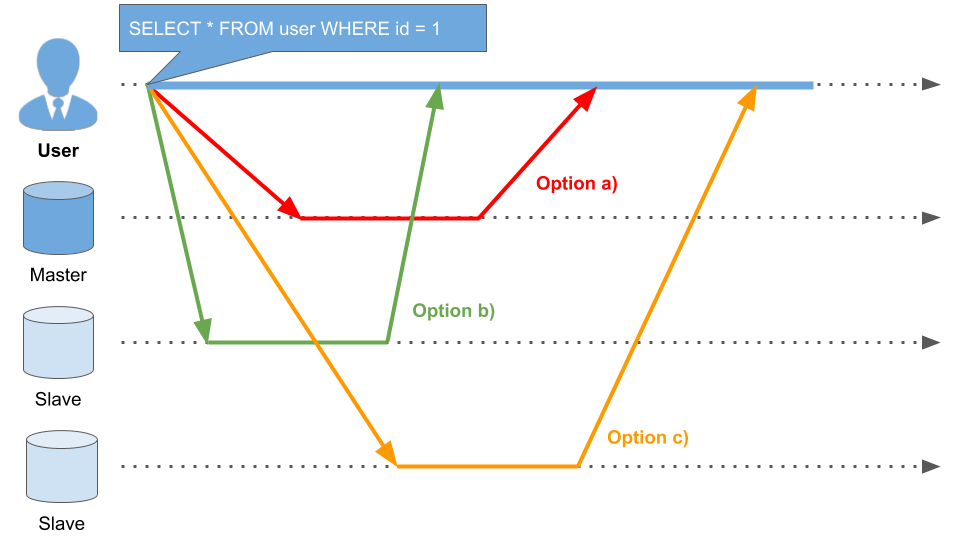
\includegraphics[width=0.8\textwidth]{replication_schema_sl_read.png}
	\caption{Schema - Master Replication - Read}
	\label{schema_replication_sl_read}
\end{figure}

Write operations as shown in Figure \ref{schema_replication_sl_write} are not that easy to handle, as only the \textit{master} is allowed to process write queries. The master processes the requests and propagates it afterwords to all slaves. When all slaves have succeeded in processing the write query, the master reports success to the user as well as making the data change visible to all other users.

\begin{figure}[H]
	\centering
  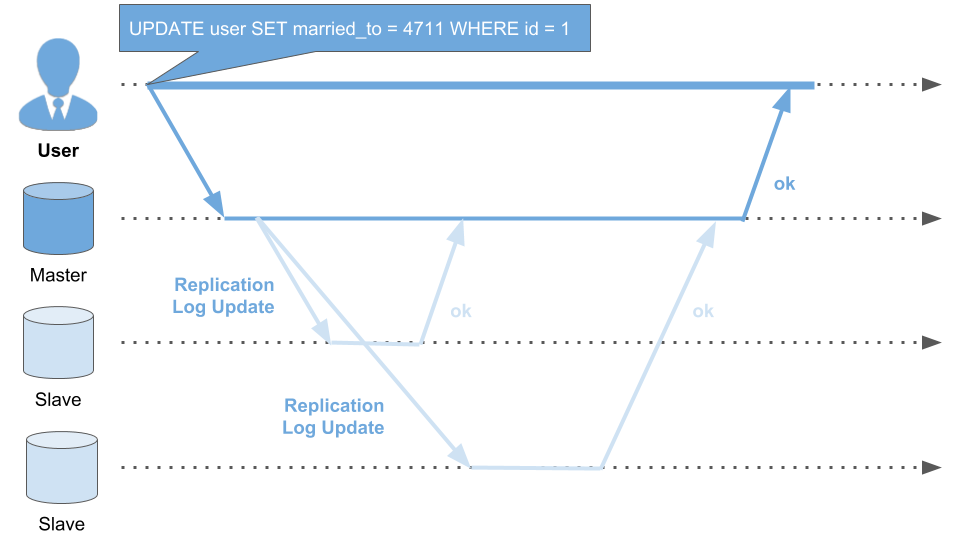
\includegraphics[width=0.8\textwidth]{replication_schema_sl_write.png}
	\caption{Schema - Master Replication - Write}
	\label{schema_replication_sl_write}
\end{figure}
\newpage

This is also calles \textit{synchronous} replication. This is usually configurable using relational databases but could also be hardcoded sometimes. There are 3 kinds of replication:\\
\begin{itemize}
\item \textbf{Synchronous:} As illustrated in Figure \ref{schema_replication_sl_write}, using synchronous replication, the master waits for slaves to succeed before reporting success to the user.
\item \textbf{Semi-Synchronous:} As illustrated in Figrue \ref{schema_replication_sl_synchronous}, using semi-synchronous replication, the master waits for one replica to report success, before reporting success to the user.
\item \textbf{Asynchronous:} The master does not wait for any slaves to report success, before reporting success to a user.\\
\end{itemize}

\begin{figure}[H]
	\centering
  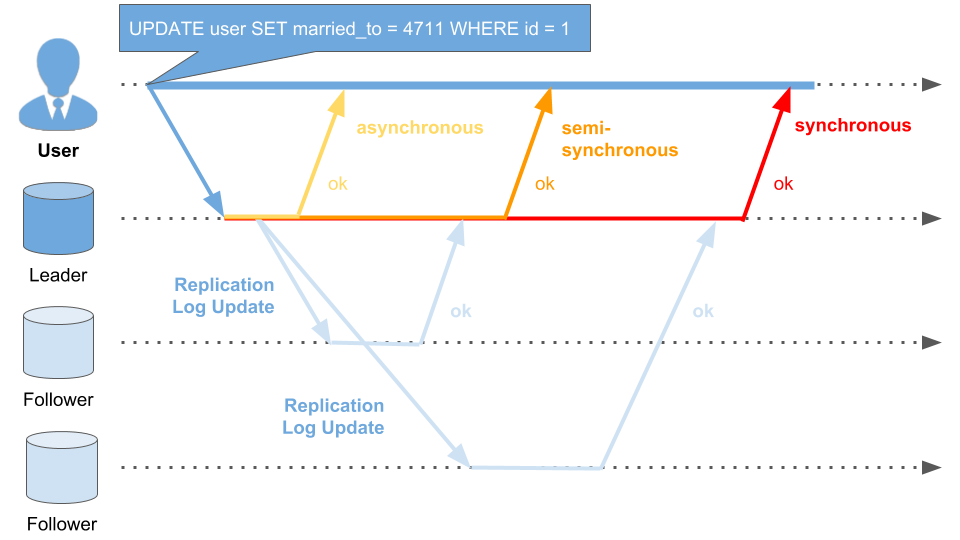
\includegraphics[width=1\textwidth]{replication_schema_sl_synchronous.png}
	\caption{Schema - Master Replication - Synchrony}
	\label{schema_replication_sl_synchronous}
\end{figure}

\textbf{Synchronous} replication ensures that all slaves have an up-to-date copy of the data that is shared with the master, which is a great advantage, as any slaves could take over if the master crashs. But this comes at a price: latency and fault tolerance. If there are networks latencies, they will directly affect the write performance, as the master needs to wait for the slaves to finish. If a slave crashs, the master won't be able to process the write query at all and waits till the replica gets available again. Even if everything is working smoothely, it will still be slower than any other replications type, as slaves still add additional processing time to write queries.\\
As you can see it usually does not make any sense to keep the whole data-system synchronous, as the failure of one node would cause the whole data-system to basically stop working. In practise it's common to make use of \textbf{semi-synchronous} replication, which means one slave is running synchronous to the master and all other slaves are running asynchronous. If the synchronous slave gets slow or crashs, one of the other asynchronous slave takes over and becomes synchronous. In this way it is guaranteed that at least two nodes store a replica which is up-to-date. This approach is much faster than the synchronous one, as one slave response is received much faster than all and probability is high, that at least one slave will be slow.\\
But there are also data systems which are completely \textbf{asynchronous} and in this way not guaranteed to ensure durability. If the master crashs and cannot be recovered, any write requests processed but not replicated to slaves, are lost. Even this is not widely used, there are cases it makes sense, as the write performance is incredibly fast and the master can still process requests, even if all slaves have failed.\\

As already spoken about \textit{performance} and \textit{scalability} at the beginning of the chapter, \textit{semi-synchronous} or \textit{asynchronous} replication is for instance a great match for achieving scalability of read-intensive data-systems. As you can distribute all read requests across multiple nodes, just by adding more \textit{slaves} nodes to the data-system, which are able to serve more read requests than a single node could handle. Beside that, getting all the benefits of data locality (like reduced \textit{latency}) comes for ``free'', as you just need to put the slave nodes geographically close to your users and consumer applications. \\
Remember it's quite unlikely a setup like this would work reliable with a data-system using \textit{synchronous} replication, as a network issue or single node failure would cause the whole data-system to be unavailable for write operations (as all writes need to be propagated to and acknowledged by every node within the data-system). Thats why most Master data-systems make use of asynchronous replication, for instance MongoDB\footnote{\cite{MDBASYNC}, https://docs.mongodb.com/manual/core/replica-set-sync/} or MySQL\footnote{\cite{MYSQLASYNC}, https://dev.mysql.com/doc/refman/8.0/en/replication.html}.\\

As you can guess, if the replication is done asynchronously, there will be a certain timeframe (\textbf{replication lag}, see Figure \ref{schema_replication_sl_replication_lag}) when the master and it's slaves will be \textit{inconsistent}, as the slaves have not yet processed the most recent write request. If you would query the modified data within this timeframe from one of the slaves, you would probably get an unexpected result. But this inconsistency is just temporary (usually just fractions of seconds depending on the \textit{load} of the data-system), if you would wait a while (without any new changes), the change will be eventually propagated to all slaves. This is also known as \textit{eventual consistency}\footnote{\cite{DBEC}}. Let's have a look at 2 examples when \textit{replication lag} is not just a theoretical issue but really causing your data-system to be inconsistent: \textbf{Reading Your Own Writes} and \textbf{Monotonic Reads}.\\

\begin{figure}[h]
	\centering
  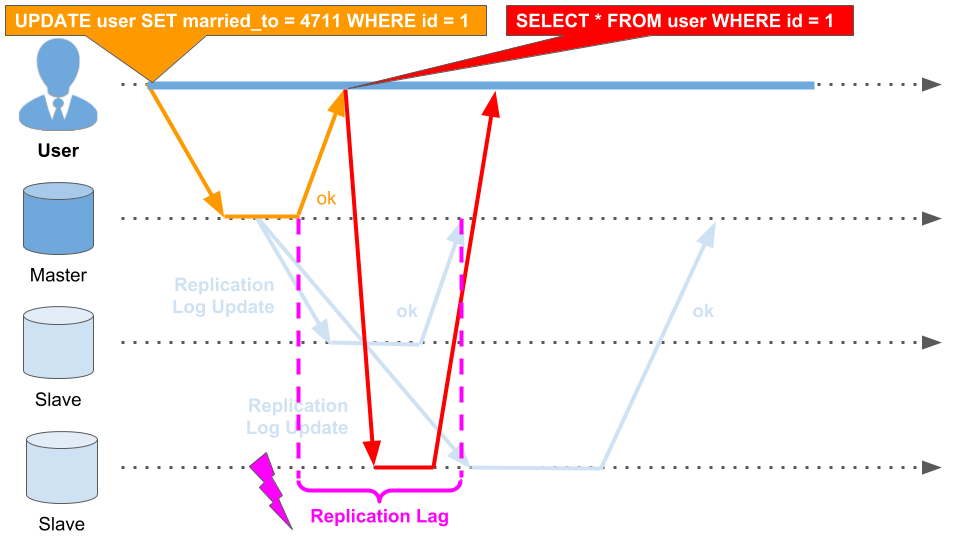
\includegraphics[width=1\textwidth]{replication_schema_sl_replication_lag.png}
	\caption{Schema - Master Replication - Replication Lag}
	\label{schema_replication_sl_replication_lag}
\end{figure}

\newpage
\subsubsubsection{Reading Your Own Writes}
You probably already know a lot of applications that let you submit or update some data and view it again later on. For instance a post to a Facebook timeline, post to a forum or something similar. In case of a master replication this submit/update request needs to be processed by the master node and propagated to all slave nodes. Using asynchronous replication it is possible that, if you query the data from a slave node (that has not yet received and processed the update), you will not get the desired result. In fact it would look like the data-system has not processed your previous write request at all (see Figure \ref{schema_replication_sl_replication_lag} on page \pageref{schema_replication_sl_replication_lag}).\\
To mitigate this issue we need \textit{read-your-writes-consistency}, which ensures that any write requests submitted by a user will directly be seen on any further read requests, guaranteeing a user his write request has been processed successfully. Approaches for achieving \textit{read-your-writes-consistency} could be, e.g.:\\

\begin{samepage}
\begin{itemize}
\item Read data, a user may have modified, from the master, otherwise make use of a slave. Using this approach you need to know, whether the required data has been modififed by a user, without querying it. For instance in case of a Xing/LinkedIn/Facebook it is pretty easy, as those profiles can only be edited by the user itself.
\item The previous approach does not work very well for data-systems where a user is able to edit almost anything of a data-system, as this would cause any read request to be executed on the master node (inhibiting scalability at all). Time or replication state could be a valuable criteria to decide wether use of he master or a slave is appropriate. The data-system could consider the time(-stamp) of the last update or processing of replication logs by slave nodes, e.g. if an update request is newer than X seconds or less than the \textit{replication lag} (all slave nodes have not yet sucessfully processed the last write request), read from master node otherwise make use of a slave node.\\
\end{itemize}
\end{samepage}
Anyhow those approaches are just some and also very simple, if you think about the same user using multiple devices: How to synchronize the last update information between both devices? How to make sure both devices connect to the same master within the same data center? What if the application does not make use of users at all?

\subsubsubsection{Monotonic Reads}
Another typical example, or rather an anomaly caused by \textit{replication lag}, is moving backward in time. This is caused by reading from asynchronous slaves. Let's take a look at Figure \ref{schema_replication_sl_monotonic_reads} as an example. Here a user runs the same read query (SELECT) twice on two different slave nodes. The first query returns up-to-date values but the second one outdated values. This happens because the user is reading from 2 different slaves, one with less and one with more replication lag, whereas the last one is still missing the replication update.\\
\textit{Monotonic Read} consistency ensures that this kind of divergence does not happen - a user will not read less recent data after reading new data. Approaches for achieving monotonic read guarantee are for instance: ensuring the same user always reads from the same replica (master or slave). Obviously different users can read from different replicas. A simple possibility to determine which replica node to read from. can be achieved by using the user id modulo the number of replica nodes - however, if a node fails, it's inevitable to reroute a users read request.\\

\begin{figure}[H]
	\centering
  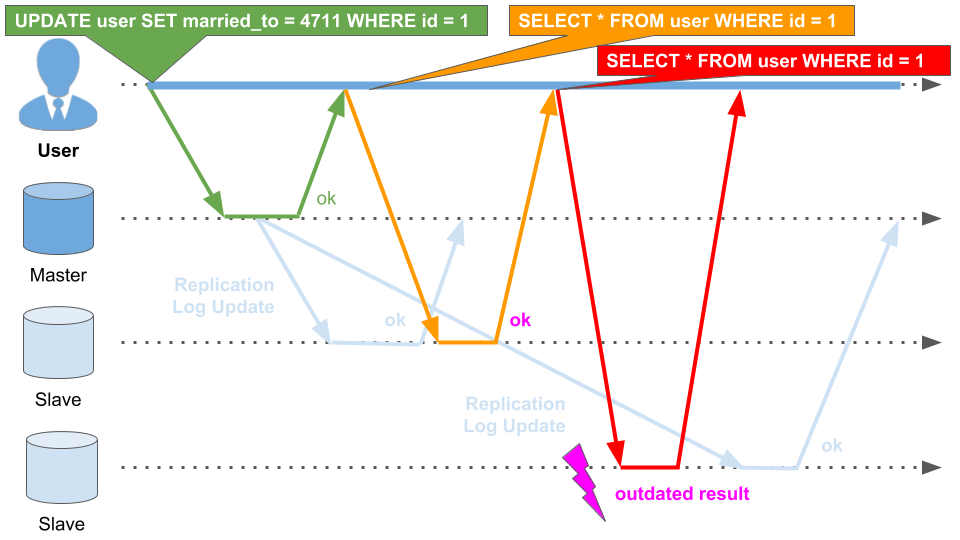
\includegraphics[width=1\textwidth]{replication_schema_sl_monotonic_reads.png}
	\caption{Schema - Master Replication - Monotonic Reads}
	\label{schema_replication_sl_monotonic_reads}
\end{figure}

\subsubsubsection{Adding New Slave Nodes}
As we have already spoken about adding new node to a replica set, due to outages of single nodes or because of the need to scale the \textit{load} of read requests horizontally. Let's take a quick look how this is usually achieved.\\
In a data-system without frequently changing datasets, it is easily done by just copying data from one node (master/slave) to the new one. But as datasets are usually changing, escpecially within the timeframe of executing the dataset copy statement, a simple copy is not appropriate, as at the end of the copy process, the new node will not be up-to-date obviously. One could think about a write lock during the execution of the copy process, but this would strongly violate our previously discussed requirement of high availability. In practise most data-systems make use of following concept:\\
\begin{enumerate}
\item \textbf{Create Snapshot:} Take a snapshot of a master or slave node (if not already done, e.g. by backup processes). Usually done by using tools of the data-system itself (e.g. Ops Manager in case of MongoDB\footnote{\cite{MDBOM}, https://docs.opsmanager.mongodb.com/current/}) or by using typical ops storage system tools for snapshotting underlying data files (e.g. LVM\abk{LVM}{Logical Volume Manager}\footnote{\cite{LVM}, http://www.sourceware.org/lvm2/} or Amazon EBS\footnote{\cite{AMZEBS}, https://docs.aws.amazon.com/de\_de/AWSEC2/latest/UserGuide/EBSSnapshots.html} for EC2 instances) or even just \lstinline{cp}/\lstinline{rsync}. It is important to notice that the last option would require to stop the data-system, running on the node the copy is taken from, as otherwise it is impossible to get a consistent snapshot. Another disadvantage of those plain copy snapshots: they are unnecessary big as they also include indexes and duplicate underlying storage padding and fragmentation.
\item \textbf{Copy Snaphsot:} Copy Snapshot to new replica slave node, for instance automatically by using tools of the data system or in a lot of cases even \lstinline{rsync} or \lstinline{cp} is used\footnote{\cite{MYSQLNS}, https://dev.mysql.com/doc/refman/5.7/en/replication-howto-additionalslaves.html}.
\item \textbf{Process Replication Log:} The new slave node connects to the master node and processes all dataset changes happened since the snapshot used, was created. This is usually done by using a replication log of the master node (e.g. \textit{Oplog} collection in case of MongoDB\footnote{\cite{MDBRSOL}, https://docs.mongodb.com/manual/core/replica-set-oplog/} or a binary \textit{relay log} in case of MySQL\footnote{\cite{MYSQLRL}, https://dev.mysql.com/doc/refman/5.7/en/slave-logs-relaylog.html}) or even slave nodes (e.g. in case of MongoDB\footnote{\cite{MDBRSOL}, https://docs.mongodb.com/manual/core/replica-set-oplog/} or MySQL\footnote{\cite{MYSQLNS}, https://dev.mysql.com/doc/refman/5.7/en/replication-howto-additionalslaves.html}). It is important to mention that the oldest entry within the replication log needs to be less recent than or equal to the creation time of the snapshot used, as the replication logs are usually capped after some time. Otherwise you would have a gap between the snaphshot and the replication log, which would lead to an information loss. A Slave which is too far behind the replication log, and in this way requirering a complete resync, is also known as a \textit{stale} slave. If this happens, you would usually need to start all over again.
\item \textbf{Go Live:} As soon as the new slave successfully processed the replication log and is up-to-date, it can start working again like any slave node, processing changes from the master as they happen.\\
\end{enumerate}

\subsubsubsection{Outages Of Nodes}
As we have already spoken about adding new nodes to a cluster, it is also important to speak about the challenge of handling node outages.\\

\textbf{Slave Outage:}\\
As previously discussed, slave nodes make use of repliation logs to stay in-sync with the master. Those replication logs and processing state (usually timestamp, number or position of event within replication log) are usually stored on the slave, for instance in case of MongoDB \textit{OpLog} (stored locally in a collection called \lstinline{local.oplog.rs}\footnote{\cite{MDBRSOL}, https://docs.mongodb.com/manual/core/replica-set-oplog/}) or in case of MySQL relay logs\footnote{\cite{MYSQLRL}, https://dev.mysql.com/doc/refman/5.7/en/slave-logs-relaylog.html}. If a slave node crashes and gets back up again or recovers from an network issue, it can just start right away where it stopped before the outage occured. It can connect to the master and request all dataset changes that have happende during the time of outage or which are newer than the last entry of the replication log before the outage. As soon as the new slave successfully processed all missing data changes and is up-to-date, it can start working again like before, processing changes from the master as they happen.\\

\textbf{Master Outage:}\\
Handling an outage of a master is not that easy, as a \textit{Failover} needs to happen: one of the replica slave nodes needs to be promoted as the new master, all other slave nodes need to consume the replication log from the new master and and clients need to send their write requests to the new master as well. A Failover can be performed manually (e.g. in case of maintenance of the master node) or automatically, which would require following 3 steps:\\

\begin{enumerate}
\item \textbf{Determining Master Failure:} As there are a lot of thing that can potentially go wrong (e.g. network, power-supply or disk outages), data-systems as well as many high-available systems make use of timeouts to identify wether a node has failed. All nodes of a data-system usually send messages (also known as \textit{Heartbeat}) between each other and if a node does not respond within a defined timeframe (e.g. 60 seconds) it is declared dead. \\
But the timeout approach also has pitfalls, for instance if the outage happened because of heavy network \textit{load}, a failover process will even increase the network load and make the whole situation much worse. This is also a reason some operation teams do not make use of automatic failover.
\item \textbf{Evaluating New Master:} There are different approaches to evaluating a new master, most common the new master is chosen by the majority of the remaining replica nodes or by a controller node (e.g. an \textit{Arbiter} node in case of MongoDB\footnote{\cite{MDBARB}, https://docs.mongodb.com/manual/core/replica-set-arbiter/}). The best candidate is obviously the one containing the most recent updates from the old master.\\
This approach has pitfalls, for instance if the cause of the outage was a network split, leaving nodes in two separate networks, not able to communicate with each other. You could end up in a \textit{split-brain} scenario, where there is a master in each network, thinking it is the only master, processing write requests and in this way corrupting all data.
\item \textbf{Reconfiguration:} As soon as the new master is elected, all clients need to send their write requests to the new master and all slaves need to receive their replication log from the new master as well. If the old master gets back up again, it needs to be ensured it recognizes the new master and will become a slave.
\end{enumerate}

\subsubsubsection{Types Of Replication Logs}
As we have already spoken a lot about replication logs, let's discuss 3 of the most common approaches:\\

\textbf{Statement-Based:}\\
Statement-based replication is the most simple approach, the master processes and afterwards adds every write request (e.g. \lstinline{INSERT}, \lstinline{UPDATE} or \lstinline{DELETE} statements in case of a relational data model) to the replication log. Those statements are later on executed by all replica slave nodes (like the master did). This approach has some pitfalls as you can guess:\\
\begin{itemize}
\item How to handle non-deterministic functions within a write request (like \lstinline{RAND()}, \lstinline{USER()} or \lstinline{NOW()} used in an SQL query) or external functions like StoredProcedures, Triggers or user-defined functions?\\
The master node would need to replace those non-deterministic functions with deterministic values (like the return value of the called function).
\item What if statements depend on other data, like in an \lstinline{UPDATE ... WHERE ...} statement. \\
This requires all statements to be executed within the exact same order, otherwise they will end up in different results.\\
\end{itemize}
As there are a lot more potential issues that need to be taken care of, today most data-systems make use of other replication log types. For instance MySQL previously made use of statement-based replication but switched to logical (row-based) replication\footnote{\cite{MYSQLRF}, https://dev.mysql.com/doc/refman/8.0/en/replication-formats.html}. But MySQL also still supports a mixed approach\footnote{\cite{MYSQLMR}, https://dev.mysql.com/doc/refman/8.0/en/binary-log-mixed.html}, which (depending of the statement) dynamically decides whether to use statement- or row-based replication. This serves the purpose of still getting the advantages of statement-based replication, like less data that needs to be written to the replication logs, which increases overall performance, especially restoring data from backups/snapshots is done more quickly.\\

\textbf{WAL (Write-Ahead-Log):}\\
Using the write-ahead-log approach, the master logs all IO data changes to a WAL (e.g. (re-)writes of disk blocks, appends to files, etc.), writes the WAL to disk and sends it to all slaves. When a slave processes this log file, it builds an exact same copy of the data structures as found at the master.\\
Using WAL results in significantly reduced IO (disk writes), because only the log file needs to be flushed to disk to guarantee that a transaction is committed, rather than every statement or data file changed by the transaction. The main disadvantage of this approach is the dependence to the used storage engine, as the WAL is very low-level and defines which byte has changed within which disk block. This makes it impossible to run different versions of a data-system or storage engine on master and slave nodes and also increases complexity of maintenance tasks, especially rolling-upgrades of single nodes within a data-system are not possible any more, making downtimes inevitable.\\
Write-Ahead-Logs are for instance used by data-systems like ArangoDB\footnote{\cite{ARANGOWAL}, https://docs.arangodb.com/3.3/Manual/Architecture/WriteAheadLog.html} or PostgreSQL\footnote{\cite{PSQLWAL}, https://www.postgresql.org/docs/9.6/static/wal-intro.html}.\\


\textbf{Logical Log Replication:}\\
Another approach for replication logs is logical (row-based) replication and unlike WAL it is decoupled from the storage engine. In case of a relational data-system a logical replication log contains records describing changes of a dataset in a row-based way:\\
\begin{itemize}
\item \textbf{INSERT:} The log contains one record with all values for each inserted row.
\item \textbf{UPDATE:} The log contains one record for each updated row as well as all new values and an information to uniquely identify the updated row (e.g. primary key).
\item \textbf{DELETE:} The log contains one record for each row to be deleted as well as information to uniquely identify the row to be deleted (e.g. primary key).\\
\end{itemize}

As this approach is decoupled from the underlying storage engine (unlike WAL), it is impossible to run different versions of the data-system or storage engine on master and slave nodes and in this way to do rolling-upgrades without the data-system having any downtime.\\

Let's take a look at an example using MongoDB. At first we switch to our desired collection (\lstinline{user}) on database \lstinline{test}, then we insert a new document containing \lstinline{user_id:1} and afterwords extending the same document by the value \lstinline{married_to:4711}:

\begin{lstlisting}[aboveskip=2ex, belowskip=2ex,emphstyle=\underbar, breaklines=true,frame=none,numbers=none,xleftmargin=0.01\textwidth,xrightmargin=0.01\textwidth,showstringspaces=false,language=java]
$ use test
 switched to db test
$ db.user.insert({user_id:1})
$ db.user.update({user_id:1}, {$set : {married_to:4711}})
\end{lstlisting}

This would lead to following replication log entries within MongoDB \textit{Oplog} (\lstinline{local.oplog.rs} collection):
\begin{lstlisting}[aboveskip=2ex, belowskip=2ex,emphstyle=\underbar, breaklines=true,frame=none,numbers=none,xleftmargin=0.01\textwidth,xrightmargin=0.01\textwidth,showstringspaces=false,language=java]
$ use local
switched to db local
$ db.oplog.rs.find()
{ 	
	"ts" : { "t" : 1534616696000, "i" : 1 }, 
	"h" : NumberLong("1342870845645633201"), 
	"op" : "i", 
	"ns" : "test.user", 
	"o" : { 
		"_id" : ObjectId("4cb35859543cc1f4f9f7f85d"), 
		"user_id" : 1 
	} 
}
{ 	
	"ts" : { "t" : 1534616699000, "i" : 1 }, 
	"h" : NumberLong("1233487572903545434"), 
	"op" : "u", 
	"ns" : "test.user", 
	"o2" : {
	 	"_id" : ObjectId("4cb35859543cc1f4f9f7f85d") 
	}, 
  	"o" : { 
  		"$set" : { "married_to" : 4711 } 
  	} 
}
\end{lstlisting}

Whereas: 
\begin{itemize}
\item \textbf{\lstinline{ts}} is the timestamp, when the operation occured.
\item \textbf{\lstinline{h}} is a unique ID of the operation. Each operation has a different value within this field.
\item \textbf{\lstinline{op}} indicates the operation to be done. (i = insert, u = update, d = delete)
\item \textbf{\lstinline{ns}} defines the database and collection affected by this operation (in our case database \lstinline{test} and collection \lstinline{user})
\item \textbf{\lstinline{o/o2}} the operation to do or in case of an insert (\lstinline{o2}) the document affected by the operation (using the docuent id).\\
\end{itemize}

If we would update multiple rows at once, MongoDB would create an entry for each row affected within the Oplog replication log.

\newpage
\subsubsection{Multi-Master Replication}
\label{tf_dds_replication_multi_master}
As we have discussed Master-based replication within the last chapter we have already noticed the biggest weakness: we have only one master. All write requests must go through it (strongly limiting write \textit{scalability}) and if the master is suffering a network outage, we are not able to process write requests anyhow. A multi-master replication  mitigates those issues, as it allows multiple (master) nodes to accept write requests. The basic replication idea of \textit{master} and \textit{slave} nodes stays the same: each master processing write requests needs to propagate those changes to all slaves as well as each master acts as a slave to the other master nodes. The multi-master replication is also known as \textit{Multi-Master}, \textit{Active/Active} or \textit{Master/Master} replication.

\begin{figure}[h]
	\centering
  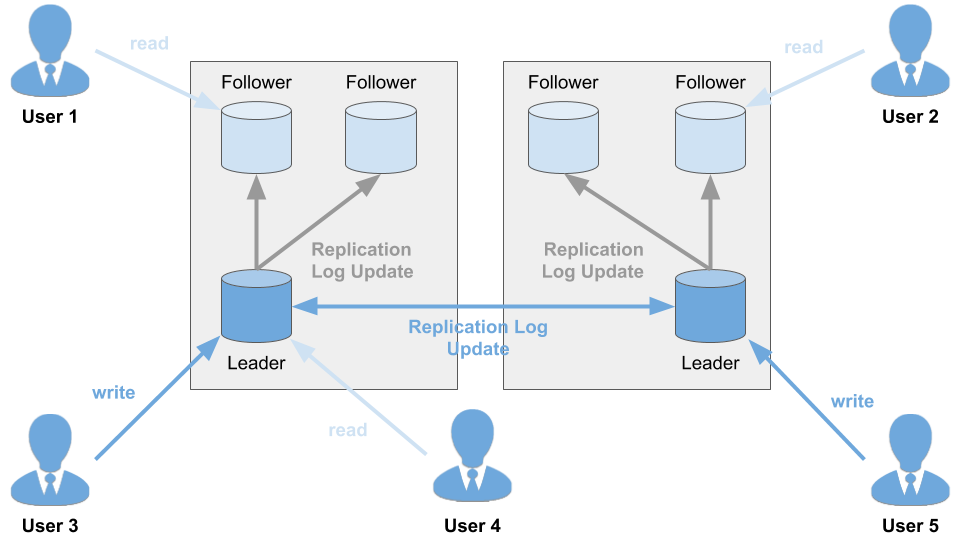
\includegraphics[width=1\textwidth]{replication_schema_ml_replication.png}
	\caption{Schema - Multi-Master Replication - Example}
	\label{schema_replication_ml_replication}
\end{figure}

Figure \ref{schema_replication_ml_replication} illustrates an example of multi-master replication setup. As you can see there are multiple master, which are able to process read requests as well as multiple slave nodes which serve the purpose of processing read requests. Using this approach approach we are able to achieve a better write \textit{performance} (\textit{horizontal scalability}) as multiple nodes are able serve read requests. In the same way the whole data-system is way more \textit{fault-tolerant} as if a single master node suffers an outage there are still other master nodes available for serving write requests (while another slave node is already in the process of being elected, replicating and replacing the old master node).\\
Implementations of multi-master replication can be found at CouchDB\footnote{\cite{CDBMM}, http://docs.couchdb.org/en/2.1.2/replication/intro.html}, PostgreSQL (using BDR\abk{BDR}{Bi-Directional Replication}\footnote{\cite{PSQLBDR}, https://www.2ndquadrant.com/en/resources/postgres-bdr-2ndquadrant/}) or MySQL (using Tungsten Replicator\footnote{\cite{TNGSTNREP}, https://github.com/continuent/tungsten-replicator} or MYSQL native multi-source implementation, which is very limited and does not even provide any conflict detection or resolution\footnote{\cite{MYSQLMS}, https://dev.mysql.com/doc/refman/5.7/en/replication-multi-source-overview.html}).\\
As also illustrated in Figure \ref{schema_replication_ml_replication} on page \pageref{schema_replication_ml_replication} a multi-master is a perfect match for setting up data-systems on multiple data-centers and getting data for read as well as write requests geographically close to users and consumer applications. But there is also a big downside using multi-master setups, as multiple nodes are able to process write requests we need to think about conflicting write requests involving the same dataset to be changed within the same time. We will discuss this within the next chapter.

\subsubsubsection{Conflicts}
Write conflicts within multi-master setups happen if the same dataset is being edited in parallel using multiple master nodes. Imagine editing the same line of a document within Google Docs simultanously: user 1 is working on a master node based in Frankfurt and user 2 is working on a master node in Berlin. Each write gets processed successfully on each master but later at the asynchronous replication between the two master nodes a conflict will arise. This won't happen if you are using a master replication. One could think about making the write requests and conflict detection synchronous, but this would be foolish as you would abandon the main benefit of multi-master replication: \textit{horizontal} write \textit{scalability}, as multiple nodes are able to process write requests. But how to handle write conflicts?\\
Well the best approach would be to avoid those conflicts, for instance this could be done by the application using the data-system. Thinking about our Google Docs example: if the application would ensure that both users are pushing their write requests to the same master, write conflicts will no longer occur.\\
But what if the application is not able to prevent those write conflicts? Let's dicsuss some common approaches for conflict resolution:\\

\begin{itemize}
\item \textbf{LWW:} as each operation has a unique ID, timestamp or both one could think about only accepting the most recent operation (Last-Write-Wins). It is important to notice that this approach is highly vulnerable to \textbf{data loss}.
\item \textbf{Merge:} merge values of multiple updates together (e.g. alphabetically or in order of appearance).
\item \textbf{Application Managed:} persist the conflict in a way, that it preserves all information without loss and let the application, using the data-system, or rather the user of the application take care about it later on (e.g. implemented by SVN\footnote{\cite{SVNWS}, https://subversion.apache.org/} or Git\footnote{\cite{GITWS}, https://git-scm.com/})
\end{itemize}


\subsubsubsection{Topologies}
If you think again about the example at the beginning of this chapter (Figure \ref{schema_replication_ml_replication} on page \pageref{schema_replication_ml_replication}) the replication topology of all master nodes is really straight forward as there are only two master nodes, which need to talk with each other. But what about setups of far more master nodes?
Figure \ref{schema_replication_ml_topologies} on page \pageref{schema_replication_ml_topologies} illustrates the most common approaches:\\
\begin{itemize}
\item \textbf{Star Topology:} one designated node acts as the single point of communication and forwards all write requests to all nodes.
\item \textbf{Circle Topology:} every node receives write operations from one node and forwards it to another node, adding its own write operations at the same time.
\item \textbf{All-To-All Topology:} every node sends it write operations to all other nodes.\\
\end{itemize} 

One issue regarding \textit{circular topology} and \textit{star topology} is, if just one node fails (in case of the star topology the center node), the whole process of master node replication is interrupted. This would not happen using \textit{all-to-all topology}. But \textit{all-to-all topology} is also vulnerable to network latencies and issues, it is not very unlikely that some write requests will overtake others in time, which requires a lot more effort in terms of conflict handling.

\begin{figure}[h]
	\centering
  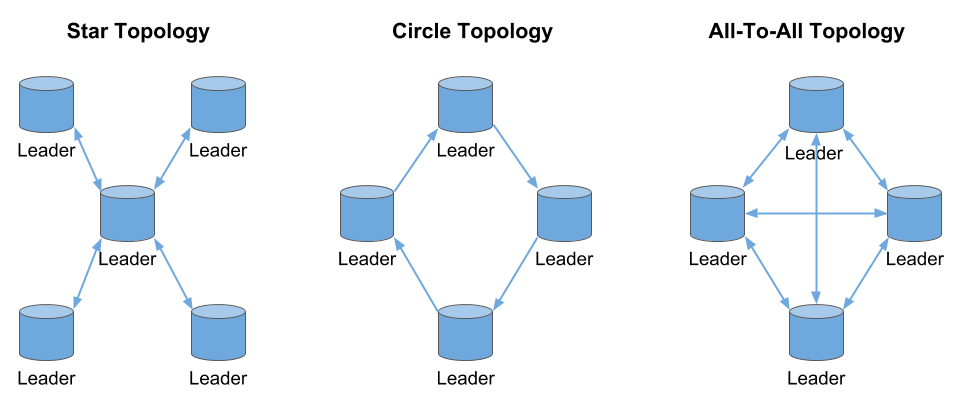
\includegraphics[width=1\textwidth]{replication_schema_ml_topologies.png}
	\caption{Schema - Multi-Master Replication - Topologies}
	\label{schema_replication_ml_topologies}
\end{figure}

\newpage
\subsubsection{Masterless Replication}
\label{tf_dds_replication_masterless}
Within the last wo chapters we have discussed (Single-/Multi-) Master-based replication, in which all write requests of users or consumer applications must go trough one or multiple dedicated master nodes. The master node will take care about propagating all changes regarding the dataset to all slave nodes. Let's take a look at another approach without any dedicated master node. \\
The basic idea of \textit{masterless replication} (also known as \textit{masterless} replication), like illustrated in Figure \ref{schema_replication_ll}, is that there is no special kind of nodes - any node will not only accept read but also write requests from clients. This approach also works very well on multiple datacenter, with respect to reasonable quorum configuration, but we will talk about that later.

\begin{figure}[h]
	\centering
  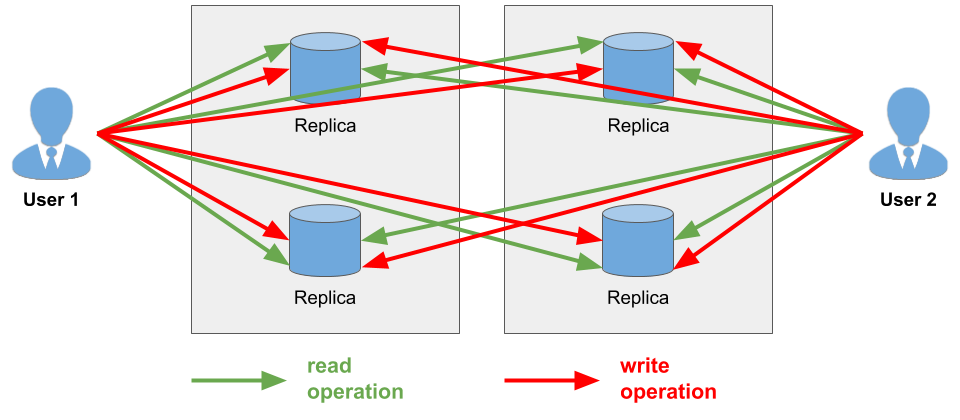
\includegraphics[width=1\textwidth]{replication_schema_ll.png}
	\caption{Schema - Masterless Replication - Example}
	\label{schema_replication_ll}
\end{figure}

Using masterless replication, clients can actual be users/consumer applications but also a \textit{controller node} in between user/consumer applications and the data-system, which acts as a proxy and takes care of routing requests.\\
For instance Cassandra makes use of an approach called \textit{coordinator} as a controller node\footnote{\cite{CASAR}, https://docs.datastax.com/en/cassandra/3.0/cassandra/architecture/archIntro.html}. Read or write requests of clients can be sent to any node within a cluster. The node receiving a request serves as the coordinator for the particular client operation. The coordinator determines which nodes within the cluster should process the request based on how the cluster is configured and which \textit{quorum} is used. This approach enables a better write performance as write requests can be parallelized as well as a better overall performance as failing and slow replica nodes can be tolerated without causing \textit{latency} and/or \textit{failover} processes. \\Other examples of data-systems using masterless replication are for instance: VoldemortDB\footnote{\cite{VOLDML}, http://www.project-voldemort.com/voldemort/design.html}, Riak\footnote{\cite{RIAKML}, http://basho.com/products/riak-kv/resiliency/} or DynamoDB\footnote{\cite{DYNML}, https://aws.amazon.com/de/dynamodb/}.\\
Data-systems using the masterless replication approach are usually able to achieve a better write \textit{performance} and \textit{horizontal scalability} as any node is able to serve write requests. In the same way the whole data-system is way more robust and \textit{fault-tolerant} than master-based approaches, as there is no \textit{single-point-of-failure} (master nodes), as multiple nodes can fail without causing the data-system being unable to serve write requests. A \textit{failover} process is not required at all, as there is no master to failover. But this comes at a price: \\
\begin{itemize}
\item The client or rather the application using the data-system needs to handle a lot of tasks a master node would usually take care of (quorum, consistency and conflict resolution)
\item Initial setup costs, as you need at least 3 nodes for a quorum to be able to ensure consistency and availability.
\item Application code complexity, as masterless data-systems usually dont provide sophisticated querying engines or basic features like referential integrity, ACID\abk{ACID}{Atomicity, Consistency, Isolation, Durability}\footnote{\cite{ACID}, ACID (Atomicity, Consistency, Isolation, Durability) is a set of properties of database transactions intended to guarantee validity even in the event of failures (network issues, hardware failures etc.}, which will force you to take care about that within your application code.
\item Almost any masterless data-system is a key/value store providing all advantages but also disadvantages and limitations of a key/value data system.\\
\end{itemize}

\newpage
\subsubsubsection{Quorums}
Let's take a look at a simple example of handling write requests on a \textit{masterless} data-system (Figure \ref{replication_schema_ll_quorum_write}). As you can see a user executes a read request, which gets distributed to all 3 replica nodes and executed in parallel. Two of three replica nodes successfully process the write requests, but one node fails (e.g. because of a failure or network outage). The overall write request returns success as at least two of the three replica nodes returne with a success message. Now what about the faulty node comes back online and starts serving read requests again, which may result in \textit{stale} (outdated) results? Let's take a look at Figure \ref{replication_schema_ll_quorum_read} on page \pageref{replication_schema_ll_quorum_read}. As you can see the read request of a user is also distribted to all replica nodes and executed in parallel. The user gets a result set of two up-to-date and one updated result, being able to determine the most recent value (\textit{last-write-wins}). \\

\begin{figure}[h]
	\centering
  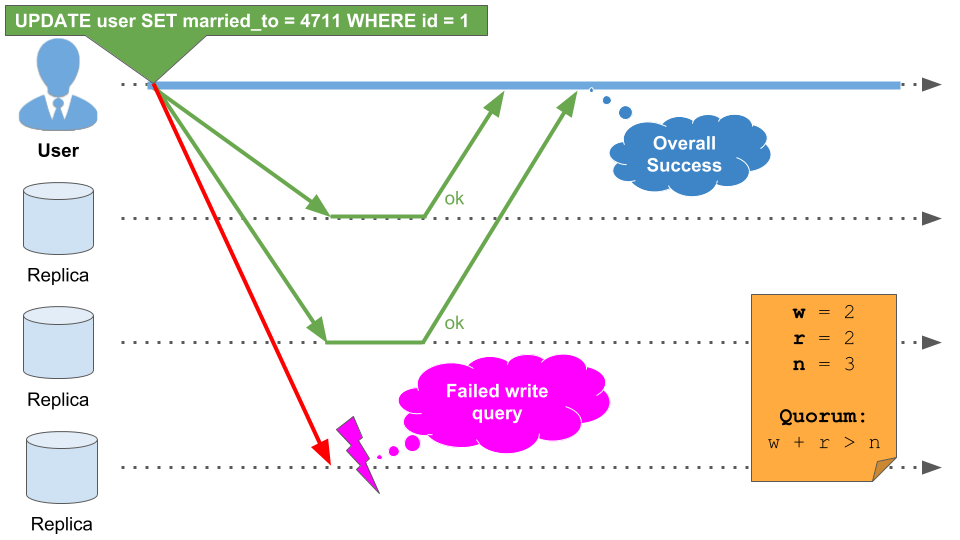
\includegraphics[width=1\textwidth]{replication_schema_ll_quorum_write.png}
	\caption{Schema - Masterless Replication - Quorum Write Example}
	\label{replication_schema_ll_quorum_write}
\end{figure}

But how to take care about outdated nodes to become eventually consistent? Let's briefly discuss 3 common approaches:\\

\begin{itemize}
\item \textbf{Read Repair:} If a user application or controller node executes a read requests and recognizes a replica node with a stale value (see Figure \ref{replication_schema_ll_quorum_read} on page \pageref{replication_schema_ll_quorum_read}), the user application or controller sends it the most recent value afterwards. For instance used by Cassandra\footnote{\cite{CASSRN}, https://docs.datastax.com/en/cassandra/3.0/cassandra/operations/opsRepairNodesTOC.html}, RIAK\footnote{\cite{RIAKRN}, http://basho.com/posts/technical/why-riak-just-works/} and VoldemortDB\footnote{\cite{VOLDML}, http://www.project-voldemort.com/voldemort/design.html}.
\item \textbf{Anti-Entropy Repair:} Some data-systems are running background processes or provide tools (e.g. \lstinline{nodetool repair} in case of Casssandra\footnote{\cite{CASSNR}, https://docs.datastax.com/en/cassandra/3.0/cassandra/tools/toolsRepair.html}) which run in background constantly looking for differences between different replica nodes and copying data from one node to another to keep everything up-to-date. For instance used by Cassandra\footnote{\cite{CASSRN}, https://docs.datastax.com/en/cassandra/3.0/cassandra/operations/opsRepairNodesTOC.html} and RIAK\footnote{\cite{RIAKRN}, http://basho.com/posts/technical/why-riak-just-works/} but not supported by VoldemortDB.
\item \textbf{Hinted Handoff:} If a node is unable to process a particular write request, the user application or coordinator node (which executed the write request) preserves the data to be written as a set of hints. As soon as the faulty node comes back online, the user application or coordinator triggers a repair process by handing off hints to the faulty node to catch up with the missed writes. For instance used by Cassandra\footnote{\cite{CASSRN}, https://docs.datastax.com/en/cassandra/3.0/cassandra/operations/opsRepairNodesTOC.html} and RIAK\footnote{\cite{RIAKRN}, http://basho.com/posts/technical/why-riak-just-works/} but not supported by VoldemortDB.\\
\end{itemize}

\begin{figure}[h]
	\centering
  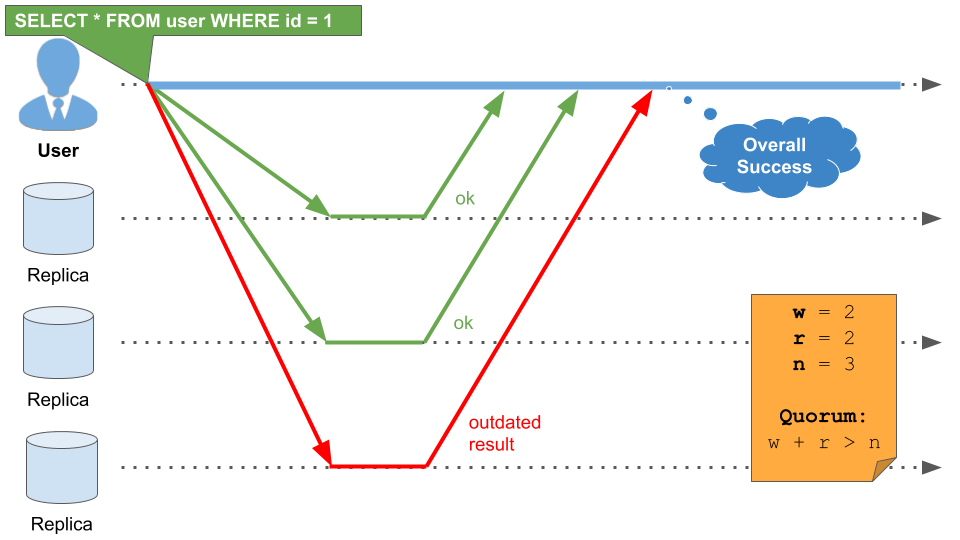
\includegraphics[width=1\textwidth]{replication_schema_ll_quorum_read.png}
	\caption{Schema - Masterless Replication - Quorum Read Example}
	\label{replication_schema_ll_quorum_read}
\end{figure}

It is important to notice that those approaches do not work like the previously discussed \textit{replication log}. Any of those repair approaches don't run in a particular order (unlike \textit{replication logs}) and there is no guarantee in terms of time when a replica node will be up-to-date again, just that it will be eventual consistent. Usually the delay is much bigger than data-systems using \textit{master-based replication}. But in terms of consistency this is totally fine as long as a reasonable quorum is used. So what is a (reasonable) quorum?\\
A quorum is the minimum number of votes that a read/write request to a distributed data-system has to obtain in order to be sure the requests is successful (and the result consistent). For instance, if a data-system has \lstinline{n} replica nodes (\lstinline{n} \textbf{is not} the number of all nodes available within the whole cluster, just the number of nodes sharing the same replica), every read and write request must be processed and confirmed by at least \lstinline{r} nodes (read) or acknowleded by at least \lstinline{w} nodes (write). A reasonable quorum is \lstinline{r + w > n}, as we can be sure to get an up-to-date result (e.g. in case of a read request) as at least one of the \lstinline{r} replica nodes will have the most-recent value for our request. Read and write requests which adhere to those rules are called \textit{quorum reads} and \textit{quorum writes}.\\
The quorum parameters are configurable, based on your cluster size, a read/write performance and fault-tolerance you want to achieve. In terms of read performance it is reasonable to choose a smaller \lstinline{r}, but resulting in a larger \lstinline{w} which causes slower writes. Vice versa a smaller \lstinline{w} will speed up writes but result in a larger \lstinline{r}, which causes slower reads. The number of node failures a data-system can tolerate can easily be calculated by:
\begin{itemize}
\item \lstinline{n - r = number} of nodes tolerated to be unavailable for read requests
\item \lstinline{n - w = number} of nodes tolerated to be unavailable for write requests \\
\end{itemize}

For instance a data-system of 5 nodes (\lstinline{n = 5}, \lstinline{r = 3} and \lstinline{w = 3}) is able to tolerate 2 unavailable nodes. 

\subsubsubsection{Limitations of Quorums}
As we discussed quorums and their advantages so for, let's have a look at some major limitations. Most quorum based data-systems allow to weaken up the quorum \textbf{r + w $\leq$ n}, for instance for the purpose of reducing \textit{latency}, increasing \textit{high availablity}, ensuring durability or just distributing the whole data-system among different datacenters, which are more closely to a user or consumer applications. This is totally fine, as long as the nodes used for read and write requests overlap at least in on node. In this way its more likely that a data-system is still able to process read and write requests, even in case of failure of multiple nodes, network or datacenter outages (unless the number of replica nodes does not get smaller than \lstinline{r} and \lstinline{w}). 
But even using the \textbf{r + w > n} quorum, there are some pitfalls resulting into reading stale values:\\
\begin{itemize}
\item \textbf{Concurrent Writes:} If two write requests are executed concurrently, it is not clear which one happened first, as both are executed from different controller nodes or applications. Both requests need to be merged, for instance based on a timestamp (\textit{last-write-wins}), which is highly vulnerable to clock skew, causing older values to overwrite more recent ones.\\
For instance Cassandra is based on \textit{last-write-wins}\footnote{\cite{CASLWW}, https://docs.datastax.com/en/cassandra/3.0/cassandra/dml/dmlWriteUpdate.html} whereas Riak requires the admin to choose whether to make use of \textit{last-write-wins} or handle write conflicts within the application using the data-system\footnote{\cite{RIALWW}, http://docs.basho.com/riak/kv/2.2.3/developing/usage/conflict-resolution/}.
\item \textbf{Concurrent Reads And Writes:} If read and write requests (regarding the same value) happen at the same time it is unclear whether the read request returns the stale or the new values. As the write request may succeeded only on some nodes during execution of the read query, the new value might be underrepresented, causing the old value to win the quorum.
\item \textbf{Node Failure:} If a node previously processed a new value, crashed and comes back online and is restored from a node with the old value, the quorum might be violated as the number of nodes storing the new value might be \lstinline{< w}.
\item \textbf{Sloppy Quorum and Hinted Handoff:} There are cases like network or datacenter outages causing some user or consumer applications being cut off from some nodes of a data-system (while the unreachable nodes are still online). In this case it is possible that some user or consumer applications won't be able to achieve a quorum. If the data-systems contains more than \lstinline{n} nodes, it needs to make a crucial decision here, whether to ignore all requests that cannot achieve a quorum or still accept write requests and just write them to some nodes outside of \lstinline{n} to ensure \textit{write availability} and \textit{durability}. A \textit{sloppy quorum} still requires \lstinline{r} and \lstinline{w} nodes, but those do not need to be one of the original \lstinline{n} nodes. As soon as the network or datacenter outage is fixed, all writes processed by nodes outside of \lstinline{n} are sent to the appropriate nodes inside of \lstinline{n} (\textit{Hinted Handoff}). Using this approach it is no longer guaranteed a data-system will provide the most recent value as read and write requests may not overlap on \lstinline{r} and \lstinline{w} nodes. This could also be mitigated by using versioning of values, like \textit{vector clocks} (e.g. used by DynamoDB\footnote{\cite{DYNVC}, https://de.wikipedia.org/wiki/Amazon\_Dynamo}).\\
For instance sloppy quorums are enabled by default within Riak\footnote{\cite{RIASQ}, http://docs.basho.com/riak/kv/2.2.3/learn/glossary/} and disabled by default within Cassandra\footnote{\cite{CASSSQ}, https://www.datastax.com/dev/blog/understanding-hinted-handoff}.\\
\end{itemize}

\subsubsubsection{Gossip}
to-be-added
\newpage
\subsection{Partitioning}
\label{tf_dds_partitioning}
Partitioning is the process of continuously dividing data into subsets and distributing it to several nodes within a data-system. Usually each record or document within a partitioned data-system is distributed and directly assigned to certain partition. We will discuss approaches on how to \textit{distribute} data and related topics like \textit{routing} of certain data and \textit{rebalancing} of nodes later within this chapter. Partitioning serves the purpose of, e.g.:\\
\begin{itemize}
\item \textbf{Scalability and Performance:} Distributing data to multiple nodes, for instance increases read/write performance and throughput as read/write queries can be distributed to multiple nodes and handled concurrently. In this way it is possible parallelize IO (disk), computing power (CPU) as well as scale the memory usage needed to run a certain operation on a part of the dataset.  
\item \textbf{Low Latency:} Using partitioning it is possible to place data close to where it is used (user or consumer applications).
\item \textbf{Availability:} Even if some nodes fail, only parts of the data are offline. \\
\end{itemize}

To avoid confusion on the term \textit{partition} or \textit{partitioning}, let's list some other terms, you might have heard and which are frequently used synonymously:
\begin{itemize}
\item \textit{shards/sharding} - (e.g. MongoDB\footnote{\cite{MDBPAR}, https://docs.mongodb.com/manual/sharding/}, ElasticSearch\footnote{\cite{ELAPAR}, https://www.elastic.co/guide/en/elasticsearch/reference/current/\_basic\_concepts.html} or RethinkDB\footnote{\cite{RDBPAR}, https://www.rethinkdb.com/docs/architecture/})
\item \textit{Vnodes/Virtual Nodes} - (e.g. Riak\footnote{\cite{RIAKPAR}, http://docs.basho.com/riak/kv/2.2.3/learn/concepts/vnodes/} or Cassandra\footnote{\cite{CASPAR}, https://docs.datastax.com/en/cassandra/3.0/cassandra/architecture/archData DistributeVnodesUsing.html})
\item \textit{region} - (e.g. HBase\footnote{\cite{HBASEPAR}, http://hbase.apache.org/0.94/book/regions.arch.html})
\item \textit{tablet} - (e.g. BigTable\footnote{\cite{BTPAR}, ``Bigtable: A Distributed Storage System for Structured Data'', Google Inc.})
\item \textit{vBucket} - (e.g. Couchbase\footnote{\cite{CBPAR}, https://developer.couchbase.com/documentation/server/3.x/admin/Concepts/concept-vBucket.html})
\end{itemize}

\begin{figure}[h]
	\centering
  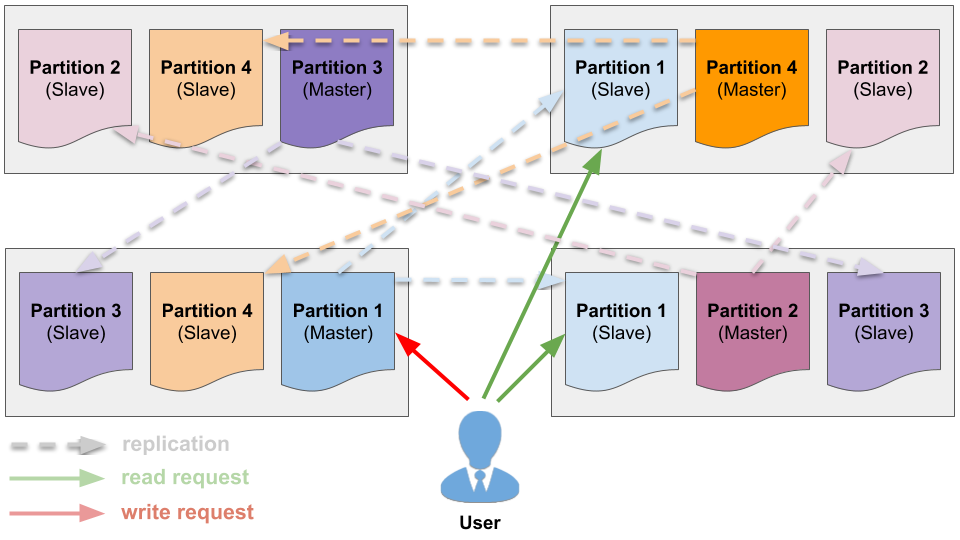
\includegraphics[width=1\textwidth]{partitioning_schema_replication.png}
	\caption{Schema - Partitioning (using Replication)}
	\label{partitioning_schema_replication}
\end{figure}

Partitioning and Replication are usually used together, especially when building data-intensive applications, as a dataset is to big to be stored on a single server or replica, and benefits of replication are required (e.g. \textit{redundancy}, \textit{fault-tolerance} or high read/write \textit{throughput}). This can be achieved by storing partitions of a data set on multiple replica nodes. In case of \textit{single-master} replication a usual approach looks like visualized in Figure \ref{partitioning_schema_replication}. Each partition is replicated to multiple nodes, it has a master node as well as 2 slave nodes storing the same data. Each single node can be a master for a certain partition but also a slave for another partition. Using this approach, datasets and \textit{load} can be easily distributed among multiple nodes as well as an outage of a node won't cause partitions to be unavailable for requests.\\[0.5 cm]

\hspace*{4mm}%
\fbox{%
  \hspace*{1.5mm}\hspace*{-1\fboxsep}%
  \parbox{0.08\textwidth + 5mm - 2\fboxsep}{%
\begin{minipage}{0.1\textwidth}
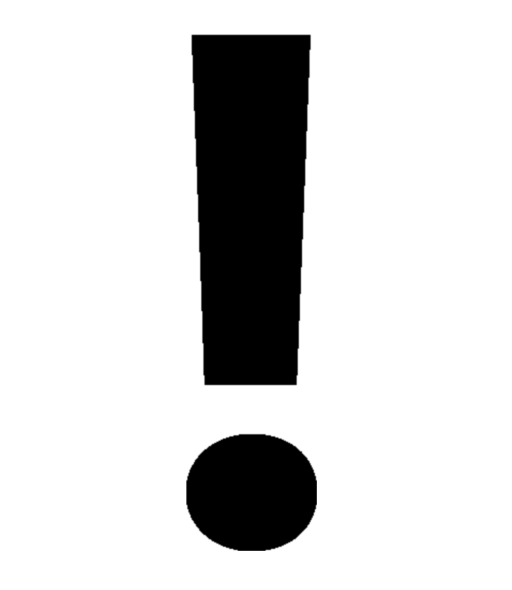
\includegraphics[width=\linewidth]{exclamation_mark.png}
\end{minipage}
  }%
}\hspace*{4mm}%
\begin{minipage}{0.8\textwidth}\raggedright
As \textbf{horizontal} and \textbf{vertical} partitioning are mixed up sometimes, it is important to notice: when we speak about partitioning within this lecture, we mean \textit{horizontal partioning}. \textit{Vertical partitioning} is an approach of traditional relational databases, usually done by splitting datasets into multiple entities (e.g. tables or databases) and using references (e.g. to achieve \textit{normalization}). \\
\end{minipage}

\subsubsection{Partitioning Of Key-Value Data}
\label{tf_dds_partitioning_key_value}
Partitioning is done with the purpose of distributing a dataset, but more important: distribute related \textit{load} (read/write queries) evenly among several nodes of a data-system. This requires the way of determining the partition of a certain row or document to be choosen wisely, as it directly affecs the performance of a data-system. An improper choosen distribution key may cause some nodes to be idle and/or empty and a single node to be the processing bottleneck and hitting its space limitations as all read/write requests end up on that single node. Whereas an appropriate distribution key will distribute the data evenly and enable the data-system to (theoretically) scale linearily in terms of space utilization and request throughput. Let's discuss some approaches for partitioning:\\
\begin{itemize}
\item \textbf{Key Range Partitioning:} Derive a partition by determining whether a key is inside a certain value range. Dicussed within chapter \ref{tf_dds_partitioning_key_value_keyrange}.
\item \textbf{Partitioning By Hash Value Of A Key:} Derive a partition by a certain hash of a given key to achieve a more even data distribution. Dicussed within chapter \ref{tf_dds_partitioning_key_value_hash_of_key}.
\item \textbf{Partitioning By List:} Every partition to be used has an assigned list of values. A related partition is derived from the input dataset by checking whether it contains one of those values. For instance all rows containing \textit{iPhone}, \textit{Samsung Galaxy} and \textit{HTC One} within a column \lstinline{device_type} are assigned to partition \textit{Smartphone}. \\
As no data-intensive system makes use of partitioning by list (as it is very improper to provide even data distribution), we wont discuss this approach in detail.
\item \textbf{Round-Robin Partitioning:} A very simple approach, which ensures even data distribution. For instance assignment to a partition can be achieved by \lstinline{n} modulo \lstinline{p} (\lstinline{n} = number of inccoming data records, \lstinline{p} = number of partitions). \\
As no data-intensive system makes use of round-robin partitioning (as for instance the direct access to an individual data record or subset usually requires accessing the whole dataset), we wont discuss this approach in detail.\\
\end{itemize}


\subsubsubsection{Key Range Partitioning}
\label{tf_dds_partitioning_key_value_keyrange}
Key Range partitioning is done by defining continues ranges of keys and assigning each of them to a certain partition. If you are aware of the boundaries of each key range, you can easily derive a partition belonging to a certain data record (and in this way node of a data-system) just by using the key of the record. This approach can be compared with an encyclopedia (compare Figure \ref{partitioning_image_wikipedia_as_book}), which is partitioned into books, of which everyone stores a certain range of articles partitioned by the first letters of the name of the article. For instance the article \textit{``Arsenal F.C.''}\footnote{https://en.wikipedia.org/wiki/Arsenal\_F.C.} will be found in partition \textit{863 ``ARS'' - ``ART''}.\\

\begin{figure}[h]
	\centering
  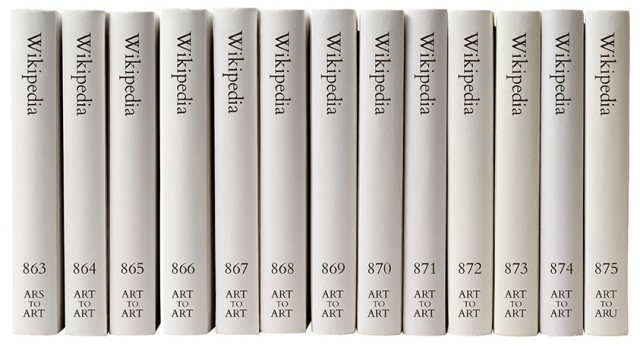
\includegraphics[width=0.8\textwidth]{wikipedia_as_book.jpg}
	\caption{Image - Wikipedia as Books}
	\label{partitioning_image_wikipedia_as_book}
\end{figure}

As you can guess a partitioning only using the first letter (\textit{A, B, C, ... Y, Z}) would lead to an unevenly data distribution. Therefore partition keys or rather boundaries need to be choosen wisely and suitable to a certain dataset, e.g. by a data-system admin or automatically. Another advantage of key range partitioning is, that some operations on a dataset are very easy, especially range scans (queries). If you partition a dataset by time (e.g. web server log files by day) it is very easy to fetch all log files related to a particular week.
Disadvantages of key range partitioning are:
\begin{itemize}
\item \textbf{Datasets Are Changing:} A key range partitioning which was suitable in the past might not be appropriate in the future. Expensive rebalancing or even repartitioning might be needed somewhen. For instance web server log files partitioned per ranges of the URL (\lstinline{/products/[A-B]}, \lstinline{/products/[C-D]}... \lstinline{/products/[Y-Z]}) maybe improper in the future, as some products will have heavier traffic than others over time (\textit{load skew}).
\item \textbf{Hotspots:} Keys that seem very appropriate in terms of even distribution at first sight, for instance partitioning of web server logfiles over time (by using timestamp of data record), create hotspots within the data system. As all write requests end up on the same partition (e.g. today), a single partition (and node(-s)) will underly heavy load whereas other partitions or rather nodes are idle (\textit{load skew}).
\item \textbf{Query Performance:} As you do not know the size of a partition beforehand, query performance is impredictable as well as partition pruning and partition-wise joins are more complex and less efficient. \\
\end{itemize}

Nevertheless for instance RethinkDB makes use of \textit{key range partitioning}\footnote{\cite{RDBARCH}, https://www.rethinkdb.com/docs/architecture/}. RethinkDB calls this approach \textit{range sharding} and its applied on the table’s primary key. If a table is configured to make use of a certain number of partitions (\textit{shards}), RethinkDB automatically examines the statistics for the table and finds the optimal set of \textit{split points} to distribute the table's data evenly among all partitions. But this comes (as discussed) at a price: every time you need to add a shard to the data-system or the dataset changes significantly over time in a way that the primary key distribution is not even anymore, you need to \textit{rebalance}\footnote{\cite{RDBREB}, https://www.rethinkdb.com/api/javascript/rebalance/} all shards of a table.

\newpage

\subsubsubsection{Hash Partitioning}
\label{tf_dds_partitioning_key_value_hash_of_key}
Hash partitioning is used to spread data efficiently and evenly among several certain partitions. This is achieved by splitting data in a randomized way rather than by using information provided within the dataset (e.g. IDs) or derived by arbitrary factors (e.g. time of data receival). The hash value itself is derived by a hash function (on a certain key of a data record) and is used to determine the partition a data records should be saved on.
\\[0.5 cm]
\hspace*{4mm}%
\fbox{%
  \hspace*{1.5mm}\hspace*{-1\fboxsep}%
  \parbox{0.08\textwidth + 5mm - 2\fboxsep}{%
\begin{minipage}{0.1\textwidth}
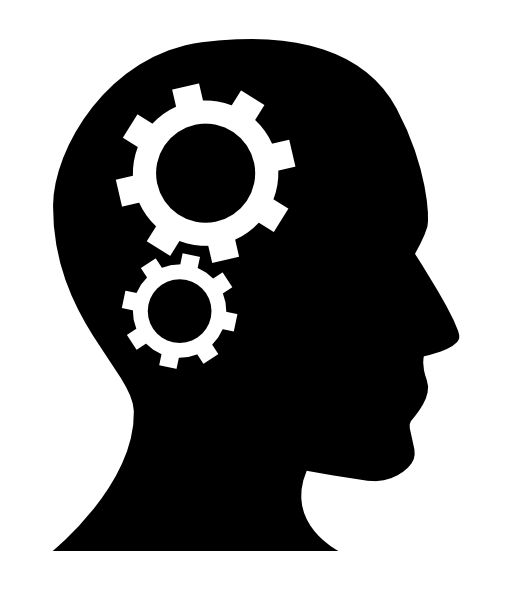
\includegraphics[width=\linewidth]{gear_brain.png}
\end{minipage}
  }%
}\hspace*{4mm}%
\begin{minipage}{0.8\textwidth}\raggedright
\textbf{Hash Function} is a function which takes input data of arbitrary size and usually provides an output of fixed size. The output of a hash function is called \textit{hash}, \textit{hash value} or \textit{digest}. A hash function needs to be \textit{deterministic} and \textit{uniform}. Common use cases for hash functions are \textit{cryptography}, \textit{checksums} and \textit{partitioning}.\\
\end{minipage}\\[0.4 cm]

Hash functions are commonly used for partitioning, as they are:
\begin{itemize}
\item \textbf{deterministic}\footnote{A deterministic hash function will provide the same output, if it is executed several times for the same input.} - as we need to be able to find records to be saved later on and 
\item \textbf{uniform}\footnote{A uniform hash function will map the inputs as evenly as possible to the available output range} - as we want to distribute the data as evenly as possible among the set of avaiable partitions and nodes, even if the inputs of the hash function (e.g. data record key) are very similar.\\
\end{itemize} 

Unlike cryptography, partitioning makes use of hash functions that are not cryptographilly strong (as this is not needed) but fast and less CPU consuming. Examples of commonly used hash function for distributed data-systems are:
\begin{itemize}
\item \textbf{MD5} - For instance used and supported by MySQL\footnote{\cite{MYSQLHP}, https://dev.mysql.com/doc/refman/5.7/en/partitioning-key.html} and Cassandra\footnote{\cite{CASHP}, https://docs.datastax.com/en/cassandra/3.0/cassandra/architecture/archPartitionerAbout.html}.
\item \textbf{MurmurHash} - For instance supported by Cassandra\footnote{\cite{CASHP}, https://docs.datastax.com/en/cassandra/3.0/cassandra/architecture/archPartitionerAbout.html}.
\item \textbf{SHA1} - For instance used and supported by Riak\footnote{\cite{RIAKHP}, http://basho.com/posts/technical/why-riak-just-works/}.
\item \textbf{CRC32} - For instance used and supported by Couchbase\footnote{\cite{CBCRC}, https://docs.couchbase.com/server/5.5/understanding-couchbase/buckets-memory-and-storage/vbuckets.html}.\\
\end{itemize} 

As an example for \textit{determinism} and \textit{uniformity} let's take a quick look at MD5 and how the hash value changes when a single character is added to the input value, when just a single character of the input value is changed or the same input value is hashed twice (see bash output in Code Snippet \ref{md5_example}).\\

\begin{lstlisting}[aboveskip=1ex, belowskip=3ex, xleftmargin=18pt, emphstyle=\underbar, breaklines=true, showstringspaces=false, captionpos=b, caption=Bash Output - \textit{MD5 Hash For Several Input Values}, label=md5_example,language=java]
marcel$ md5 -s abc
MD5 ("abc") = 900150983cd24fb0d6963f7d28e17f72
// add a single character ("d")
marcel$ md5 -s abcd
MD5 ("abcd") = e2fc714c4727ee9395f324cd2e7f331f
// change  a single character ("d" to "e")
marcel$ md5 -s abce
MD5 ("abce") = b9c4fe92c2a30ef69833ac8f53eebcec
// hash again with same input value
marcel$ md5 -s abce
MD5 ("abce") = b9c4fe92c2a30ef69833ac8f53eebcec
\end{lstlisting}

As you can see \textit{uniformity} is ensured, as with just the change of a single character the resulting hash is completely different. \textit{Determinism} is also fulfilled as executing the function with the same input value produces the same hash value.\\
Using this hash functions, distributed data-systems are able to distribute records among partitions, this is usually done by two common approaches:\\

\textbf{Hash Modulo:}\\ 
Take the calculated hash value \textit{V} and calculate \textit{V} \lstinline{modulo} \textit{N} (number of partitions). This allows the the data-system to easily distribute and receive records to and from a given number of partitions. Unfortunately this approach has a major disadvantage in terms of \textit{scalability} especially \textit{operability}. As data-systems usually grow significantly over time (which requires adding additional nodes (\textit{N}) to a data-system to cope with the increasing data volume) \textit{hash modulo} causes a lot of trouble, as an increased (as well as decreased) \textit{N} results in different partition assignments for a lot of records (depending on size of \textit{N}), which will require to shuffle and reassign already saved data again among all partitions. That's the main reason most data-systems we talk about within this lecture (unlike traditional databases) do not make use of \textit{hash modulo} but \textit{consistent hashing}. Nevertheless for instance elasticsearch makes use of it, a partition (called \textit{shard}) is derived by\footnote{\cite{ESROUT}, https://www.elastic.co/guide/en/elasticsearch/guide/current/routing-value.html}:
\begin{lstlisting}[aboveskip=2ex, belowskip=2ex,emphstyle=\underbar, breaklines=true,frame=none,numbers=none,xleftmargin=0.15\textwidth,xrightmargin=0.15\textwidth,showstringspaces=false,language=java]
shard = hash(routing) % number_of_primary_shards
\end{lstlisting}
The number of shards for an \textit{index}\footnote{index - An index is a collection of documents. Compared to a relational database like MySQL: elasticsearch can contain multiple indices (databases), which in turn contain multiple types (tables). These types hold multiple documents (rows), and each document has properties (columns).} can increased (by \lstinline{_split}\footnote{\cite{ESSPLIT}, https://www.elastic.co/guide/en/elasticsearch/reference/6.4/indices-split-index.html}) or decreased (by \lstinline{_shrink}\footnote{\cite{ESSHRINK}, https://www.elastic.co/guide/en/elasticsearch/reference/6.4/indices-shrink-index.html}) some time after creation but this is not a trivial task and will usually require recreating the same or even creating a new \textit{index}.\\


\textbf{Consistent Hashing:}\\  
Assign a range of hashes to every partition (and in this way node). Every record will be stored and read from the partition in charge for a given range of hash values. Imagine \textit{consistent hashing} as a ring of keys (see Figure \ref{partitioning_consistent_hashing} on page \pageref{partitioning_consistent_hashing}). Each node (\textit{N\textsubscript{\textbf{i}}}) is in charge for serving all hash values \textit{v} in between \textit{i} and the position \textit{j} of its clockwise predecessor \textit{N\textsubscript{\textbf{j}}} :\\
\centerline{\textbf{j < v $\leq$ i}}

Using \textit{consistent hashing} even distribution and avoiding of hotspots is also ensured by using hash values of keys. Unlike \textit{hash modulo} this approach is not vulnerable for a changing cluster size (number of nodes \textit{N}), as for instance in case of removing a node (see Figure \ref{partitioning_consistent_hashing} on page \pageref{partitioning_consistent_hashing}, node 7), the higher neighbour (node 8) takes over and all other data does not need to be touched or reassigned. Node \textit{N\textsubscript{\textbf{8}}} is no longer in charge of hash values \textit{v} between \textbf{7 < v $\leq$ 8} but \textbf{6 < v $\leq$ 8}. 

\begin{figure}[h]
	\centering
  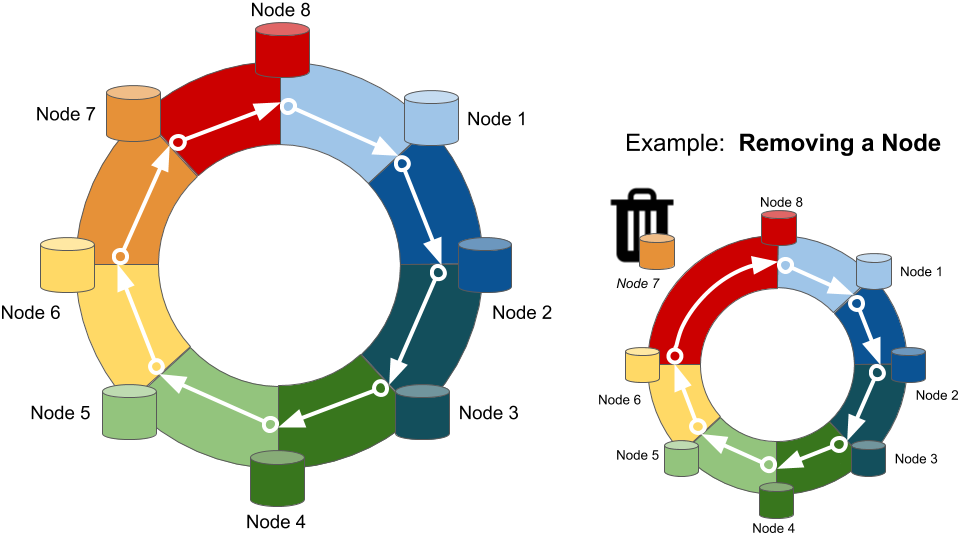
\includegraphics[width=1\textwidth]{partitioning_consistent_hashing.png}
	\caption{Schema - Consistent Hashing}
	\label{partitioning_consistent_hashing}
\end{figure}

In case of a node is added to the data-system, it just takes values from another node and all other partitions and nodes do not need to be touched. As you can see after every addition or removal of a node, only \textit{c}/\textit{N} keys need to be redistributed (where \textit{c} is the count of hash values and \textit{N} is the number of nodes within the data-system). Because of that \textit{cosistent hashing} has become a de facto standard for all modern highly distributed data-systems (e.g. Cassandra\footnote{\cite{CASCH}, https://docs.datastax.com/en/cassandra/3.0/cassandra/architecture/archDataDist ributeHashing.html}, Riak\footnote{\cite{RIAKCH}, http://docs.basho.com/riak/kv/2.2.3/learn/glossary/}, VoldemortDB\footnote{\cite{VDBCH}, http://www.project-voldemort.com/voldemort/design.html} or DynamoDB\footnote{\cite{DYNDBCH}, https://cloudacademy.com/blog/dynamodb-replication-and-partitioning-part-4/}).\\

It is important to notice a disadvantage of \textit{consistent hashing}: range queries. As keys are now randomly distributed among all partitions (to achieve even distribution) range queries will perform less efficient compared to \textit{key range partitioning} as the query needs to be sent and processed by all partitions (and therefore nodes). For instance MongoDB provides \textit{key range partitioning} (called \textit{ranged sharding}\footnote{\cite{MDBRS}, https://docs.mongodb.com/manual/core/ranged-sharding/}) as well as \textit{hash partitioning} (called \textit{hashed sharding}\footnote{\cite{MDBHS}, https://docs.mongodb.com/manual/core/hashed-sharding/}) to efficently serve both use cases, but you still need to choose wisely and make a trade-off which one to use depending on your case.\\

\newpage

\subsubsection{Partitioning Of Secondary Indices}
\label{tf_dds_partitioning_secondary_indices}

We previously discussed partitioning mostly relying on key-value data, in which a single key is not only used for partitioning but also as the primary key of a dataset. If you only need to access the data by the primary key, determination of the belonging partition can easily be achieved by using the hash function as described within the last chapter. But what if you need to access the data by attributes within a record or even do a range scan on those attributes? Let's take our previous discussed Example of Facebook profiles as an example (Figure \ref{schema_facebook_relational_model} on page \pageref{schema_facebook_relational_model}). If you want to receive a single profile and know the \lstinline{user_id}, a belonging partition can easily be determined, but if you want to receive all profiles of people living in ``\textit{Palo Alto}'' \textit{secondary indices} are a good choice to efficiently access the required data by attributes that are other than the primary key. \\
You probably already know the idea of \textit{secondary indices} from traditional relational databases like DB2, Oracle or Informix discussed within previous lectures. Applying this concept on distributed data-systems is a little bit more complex, as \textit{secondary indices} need to take care of partitions of the data they link to as well as they even need to be partioned themself too. We will take a closer look on two common approaches for \textit{secondary indeces} and partitioning within the next two chapters \textit{\ref{tf_dds_partitioning_secondary_indices_local_index} \nameref{tf_dds_partitioning_secondary_indices_local_index}} and \textit{\ref{tf_dds_partitioning_secondary_indices_global_index} \nameref{tf_dds_partitioning_secondary_indices_global_index}}.

\subsubsubsection{Local Secondary Indices}
\label{tf_dds_partitioning_secondary_indices_local_index}

A \textit{local secondary index} (also known as \textit{LSI}\abk{LSI}{Local Secondary Index}) is achieved by creating, storing and maintaining the index locally in every partition. Insert, update or delete operations are performed locally on the node and partition the index belongs to. Every partition basically manages its own index and all pointers reference to local data items. For instance if a data record is added to a partition, the partition also automatically adds the new entry to its secondary index. Maintaining a local index requires less overhead and is in this way usually much faster than maintaining a global index. But do not ignore that maintaining the local index will compete with the local workload and affect the throughput and if your cluster grows significantly in size (amount of nodes), \textit{scattering} and \textit{gathering} overhead will probably have a major impact on read request performance.\\
Let's get back to the previously mentioned example of Facebook profiles (Figure \ref{schema_facebook_relational_model} on page \pageref{schema_facebook_relational_model}) and how this would look like using \textit{local secondary indices}: Figure \ref{partitioning_secondary_indexes_local} on page \pageref{partitioning_secondary_indexes_local}. As you can see every partition has its own local secondary indices. If you for instance want to query alle profiles of people living in ``\textit{Palo Alto}'', you would need to query the secondary index of every partition (\textit{scatter} and \textit{gather}) as the data is not partitioned by \lstinline{city} and related entries can be found in any partition. This is also a major weakness of \textit{local secondary indices}, as they are expensive as you need to query all partitions. This can be done in parallel, as we are talking about distibuted, partitioned and probably replicated data-systems but you should keep that always in mind. It is recommended to partition a dataset in such a way, secondary indices can be served by one partition, but thats not always feasible. especially if you make use of multiple seconday indices within one query.\\
\textit{Local secondary indices} are implemented and provided by e.g. Riak\footnote{\cite{RIAKSIL}, http://docs.basho.com/riak/kv/2.2.3/using/reference/secondary-indexes/}, Cassandra\footnote{\cite{CASSIL}, https://www.datastax.com/dev/blog/cassandra-native-secondary-index-deep-dive} and DynamoDB\footnote{\cite{DYNDBSIL}, https://docs.aws.amazon.com/amazondynamodb/latest/developerguide/LSI.html}.

\begin{figure}[h]
	\centering
  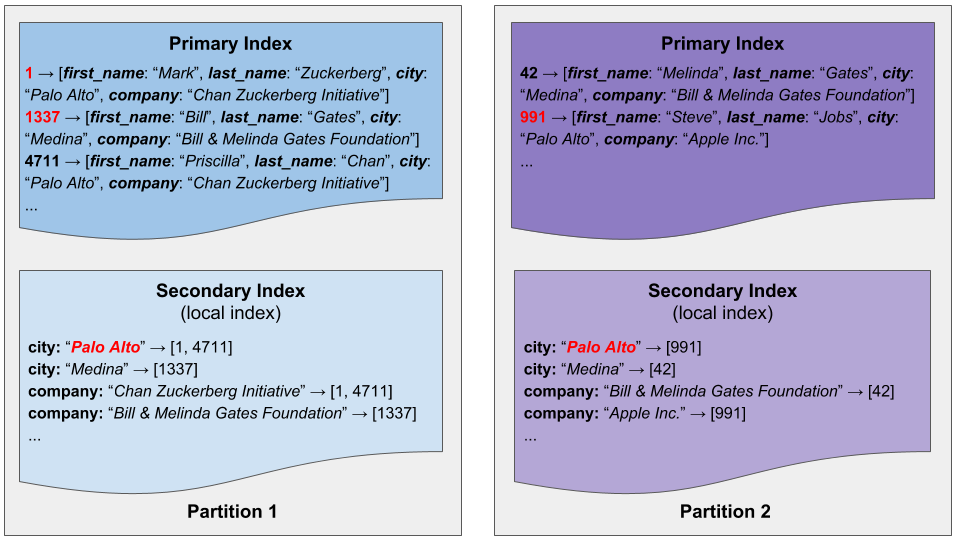
\includegraphics[width=1\textwidth]{partitioning_secondary_indexes_local.png}
	\caption{Schema - Secondary Indices (local)}
	\label{partitioning_secondary_indexes_local}
\end{figure}

\newpage

\subsubsubsection{Global Secondary Indices}
\label{tf_dds_partitioning_secondary_indices_global_index}

A \textit{global secondary index} (also known as \textit{GSI}\abk{GSI}{Global Secondary Index}) is achieved by creating, storing and maintaining the index globally and independent of local data items of partitions. Insert, update or delete operations require remote updates of the index for the belonging data. A \textit{global secondary index} could be saved on a single node but that would not only violate the basic idea of distributed data-systems, \textit{scalability} and \textit{reliability} but also will also be impossible at some time as the size of the index gets to big for one node. So every \textit{global secondary index} is partitioned by its own key indepent of local data records. For instance if a data record is added to a partition, the partition also automatically adds the new entry to its secondary index.\\ 
Maintaining a global index requires more overhead and is in this way usually slower than maintaining a local index but also more efficent in terms of read requests as you only need to query one partition index instead of \textit{scattering} and \textit{gathering} all partitions. This approach usually weakens the read consistency, as indices updates take more time, for instance DynamoDB supports \textit{strong consistency} for \textit{local secondary indices}\footnote{\cite{DYNDBSIL}, https://docs.aws.amazon.com/amazondynamodb/latest/developerguide/LSI.html} but only \textit{eventual consistency} for \textit{eventual consistency} for \textit{global secondary indices}\footnote{\cite{DYNDBGIL}, https://docs.aws.amazon.com/amazondynamodb/latest/developerguide/GSI.html}.\\
\textit{Local secondary indices} are mostly implemented by traditional relational databases (e.g. Oracle Database\footnote{\cite{ORCLGSI}, https://docs.oracle.com/database/121/VLDBG/GUID-EE7C7B09-81BD-4996-8AC1-42A50D26FC25.htm} or Microsoft SQL Server\footnote{\cite{MSSQLGSI}, https://docs.microsoft.com/de-de/sql/relational-databases/partitions/partitioned-tables-and-indexes?view=sql-server-2017}) but rarely used by BigData data-systems. Nevertheless DynamoDB\footnote{\cite{DYNDBGIL}, https://docs.aws.amazon.com/amazondynamodb/latest/developerguide/GSI.html} and Couchbase\footnote{\cite{CBGSI}, https://docs.couchbase.com/server/5.5/indexes/indexing-overview.html} make use of them.\\

\begin{figure}[h]
	\centering
  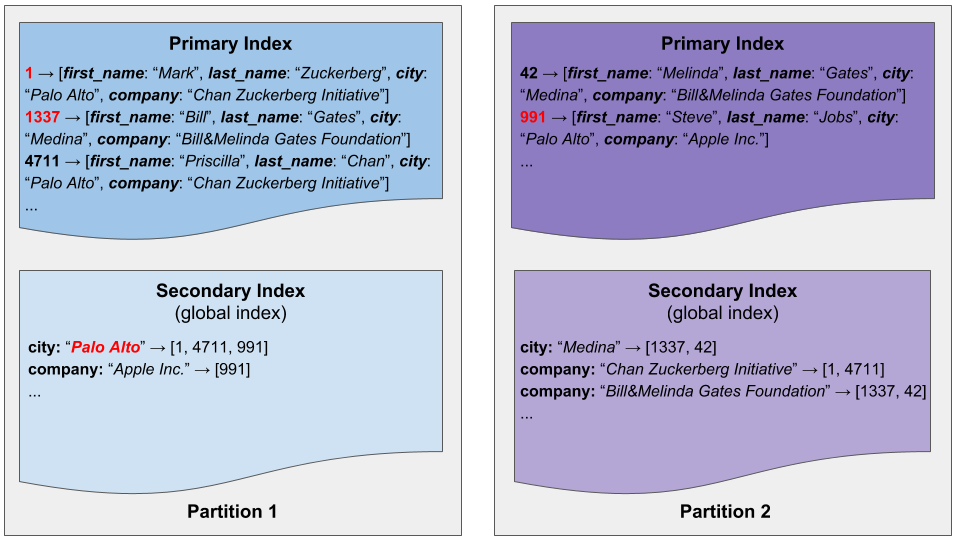
\includegraphics[width=1\textwidth]{partitioning_secondary_indexes_global.png}
	\caption{Schema - Secondary Index (global)}
	\label{partitioning_secondary_indexes_global}
\end{figure}

Let's get back to the previously mentioned example of Facebook profiles (Figure \ref{schema_facebook_relational_model} on page \pageref{schema_facebook_relational_model}) and how this would look like using a \textit{global secondary index}: Figure \ref{partitioning_secondary_indexes_global} on page \pageref{partitioning_secondary_indexes_global}.
As you can see every \textit{global secondary index} is partioned and stored complety independant of the belonging data it points to. If you for instance want to query alle profiles of people living in ``\textit{Palo Alto}'', you would query the secondary index of partition 1 once and be able to get all related records, irrespective of which partition they are stored in. The \textit{global secondary index} itself is also partitioned, as you can see, but completely independent of the partions of the data records it points to. \\
This approach is usually faster in terms of read requests, as you only need to query one partition to get the full secondary index instead of \textit{scattering} over all partitions. But it could also be slower at write operations, as if only one record changes, probably multiple indexes and partitions (probably on multiple nodes) need to be updated too.
\newpage

\subsubsection{Rebalancing Partitions}
\label{tf_dds_partitioning_rebalancing}

\subsubsection{Request Routing}
\label{tf_dds_partitioning_request_routing}


\subsection{Transactions}
\label{tf_dds_transactions}
to-be-added

\subsection{Consistency}
\label{tf_dds_consistency}
to-be-added